\documentclass[13pt, letterpaper, oneside]{book}
\usepackage{graphicx}

\usepackage[driver=xetex,paperwidth=8.5in,paperheight=11in,left=1.4in,
right=1in,top=1.3in, bottom=1.4in]{geometry}
\usepackage[no-math, quiet]{fontspec}
\usepackage{newfloat}
\usepackage{sectsty, tikz, color, pgfplots}
\usetikzlibrary{shapes,arrows}
\usepackage{multicol}
\usepackage{amsmath, amssymb, amsfonts, amsthm, titlesec}
\usepackage[urw-garamond,cal=cmcal]{mathdesign}
\usepackage{fancyhdr, booktabs, longtable}
%\usepackage[font=small,format=plain,labelfont=it,textfont=it]{caption}
\usepackage{caption,subcaption}
\usepackage{listings}
\usepackage{algpseudocode, algorithm,setspace}
% \usepackage[T1]{fontenc} 
\usepackage{enumitem,verbatim,natbib}

\usepackage{changepage}
 \DeclareTextCommandDefault{\nobreakspace}{\leavevmode\nobreak\ } 

%========== DEFINITIONS ==========

\newlist{alist}{itemize}{1}
\setlist[alist]{label=--,labelindent=2in,leftmargin=9pt,labelsep=6pt, itemsep=0pt}

\def\Lmax{L_{\text{max}}}
\def\est{\mathtt{est}}
\def\lst{\mathtt{lst}}
\def\eft{\mathtt{eft}}
\def\lft{\mathtt{lft}}
\def\startOf{\mathtt{startOf}}
\def\endOf{\mathtt{endOf}}

%=========== TIKZ STUFF =========

\usetikzlibrary{fit}
\makeatletter
\tikzset{
  fn/.style={
    inner sep=0pt,
    fill=none,
    draw=none,
    reset transform,
    fit={(\pgf@pathminx,\pgf@pathminy) (\pgf@pathmaxx,\pgf@pathmaxy)},
  },
  reset transform/.code={\pgftransformreset}
}
\makeatother

%========= ALGO STUFF ============

%========= FONT SPECS ============
\tolerance 8000

\defaultfontfeatures{Mapping=tex-text, Ligatures=Common}

%\renewcommand\refname{references} % this sets the name of
\def\labelitemi{--}

\def\sansfont{\fontspec[Script=Latin,LetterSpace=2.6, Mapping=tex-text]{DIN 1451 Mittelschrift}}
\def\sansitalicfont{\fontspec[Script=Latin,LetterSpace=2.6, FakeSlant=0.2, Mapping=tex-text]{DIN 1451 Mittelschrift}}

\def\monofont{\fontspec[Script=Latin,Mapping=tex-text,Scale=0.91, AutoFakeBold]{Inconsolata}}

\renewcommand{\texttt}[1]{{\monofont #1}}
\renewcommand{\mathtt}[1]{{\text{\monofont #1}}\,}

\renewcommand{\normalsize}{\fontsize{12pt}{16pt}\selectfont}

%========== COLOR STUFF ===============

\definecolor{darkred}{rgb}{0.6, 0, 0.00}


%============ LISTINGS ==============
\lstset{
aboveskip=2\medskipamount, belowskip=2\medskipamount,
basicstyle=\monofont,
language=python,
numbers=left, numberstyle=\tiny,  numbersep=9pt,
xleftmargin=.4in, frame=l, xrightmargin=1.74in
}


%============= PAGE LAYOUT ============

%\titleformat{\section}{\huge\sansnormalfont}{\protect\makebox[0pt][r]{\thesection\quad}}{0em}{}
\titleformat{\chapter}{\fontsize{32pt}{36pt}\selectfont\sansfont}{}{0em}{}
\titleformat{\section}{\fontsize{18pt}{22pt}\selectfont\sansfont}{\protect\makebox[0pt][r]{\thesection\quad}}{0em}{}
\titleformat{\subsection}{\fontsize{12pt}{16pt}\selectfont\sansfont}{\protect\makebox[0pt][r]{\thesubsection\fontsize{18pt}{22pt}\selectfont\quad}}{0em}{}
%\titleformat{\paragraph}{\fontsize{12pt}{16pt}\selectfont}{}{}{}


\fancyhead[LE]{\sansfont\small Scheduling non-identical jobs on a batch resource \normalsize}
\fancyhead[RE]{}
\fancyhead[LO]{}
\fancyhead[RO]{\sansfont\small \nouppercase\rightmark}
\fancyfoot[C]{\sansfont\thepage}

\fancypagestyle{plain}{
\fancyhf{}
\renewcommand{\headrulewidth}{0pt}
\fancyfoot[C]{\sansfont\thepage}
}

%====== CHAR REPLACEMENTS ======%
\let\oldemptyset\emptyset
\let\emptyset\varnothing

%===== LONG EQUATION THINGS =====%
\DeclareFloatingEnvironment[
  fileext=los,
  listname=List of Models,
  name=Model,
  placement=tbhp,
  within=section
]{model}



\widowpenalty 300
\clubpenalty 300

\usepackage[hidelinks]{hyperref}

\begin{document}

\fontsize{12pt}{16pt}\selectfont
\thispagestyle{empty}
\pagestyle{fancy}

\vskip 5em
\begin{centering}

\LARGE\sansfont{Scheduling non-identical jobs on a batch resource}

\vspace{1.2em}
\large
\sansfont by \\ Sebastian Kosch\\

\vspace{5.2em}

\normalfont\fontsize{12pt}{16pt}\selectfont

Supervisor: Prof. J. Christopher Beck

April 2013

\end{centering}

\pagebreak

\frontmatter

\thispagestyle{empty}
\vspace*{\fill} %blank flyleaf
\pagebreak
\fontsize{12pt}{16pt}\selectfont
\thispagestyle{empty}
\pagestyle{fancy}

\baselineskip=16.8pt plus 0pt
\frenchspacing

\begin{centering}
\vspace{3em}
\LARGE\sansfont{Scheduling non-identical jobs on a batch resource}

\vspace{2em}
\large
\sansfont Sebastian Kosch\\

\vfill
\normalfont
\fontsize{12pt}{16pt}\selectfont
A thesis submitted in conformity with the requirements

for the degree of \textit{Bachelor of Applied Science}

\vspace{1em}
Supervisor: Prof. J. Christopher Beck, MIE

\vspace{2em}

\textmd Division of Engineering Science\\
University of Toronto\\

April 2013

\end{centering}
\pagebreak

% abstract
\pagebreak

\frontmatter
\chapter*{Abstract}
Ovens, washers, driers and autoclaves, as examples of \textit{batch processing
machines}, are used in many industries. We examine the problem of
scheduling jobs of non-identical sizes, processing times and due dates on a
single batch machine of finite capacity in a way that minimizes the maximum
lateness $\Lmax$. Previous authors have introduced a branch-and-price method and
a new global constraint for constraint programming solvers, both of which
perform better than a simple mixed-integer program. In this paper, we
present four new models: an improved version of the mixed-integer program, a
simple constraint programming model, a decomposition approach and a new
mixed-integer model using a novel way to compute batch lateness. All models are
evaluated on a set of problem instances and compared by performance. We show
that the new mixed-integer model rivals the performance of the previously
introduced global constraint.

% acknowledgements
\pagebreak
\vspace*{\fill}

\begin{adjustwidth}{1in}{1in}

  I must acknowledge Professor Chris Beck, one of the best teachers I
  have had, who took considerable time out from his busy schedule to keep me on track throughout the year.
  
  Thank you for being a model supervisor.\\[3ex]
     And I could not have made it this far without two incredible parents and
     without QP.
     
     I love you guys.
\end{adjustwidth}
    \vspace*{\fill}
%\include{firstpage}

\tableofcontents
\listoffigures
\listoftables

\pagestyle{fancy}
\mainmatter
\pagebreak
\vskip 4em
\fontsize{12pt}{17pt}\selectfont
\chapter{Introduction}
This paper discusses four different approaches, and several variations on them,
to solving the problem of scheduling non-identical jobs on a batch processing
machine. Batch processing machines, for the purposes of this paper, can process
multiple, non-identical jobs simultaneously---but all jobs must be loaded into
and unloaded from the machine at once, which introduces a considerable twist on
the ``simple parallel resources'' known from typical example problems in
existing literature.

The machines in question represents real-life resources like autoclaves or
ovens, which can process multiple items at a time, but often cannot be opened at
random---in fact, such machines often need to wait for the largest item in the
batch to be done before the next batch can be inserted.

\citet{Malapert} proposed a global constraint programming (CP) algorithm consisting
of a set of filtering rules to solve the problem. He achieved considerably
better speeds than with a simple mixed-integer model (MIP), but it seems plausible
that the new global constraint is more cumbersome than necessary to achieve this
performance; simple MIP, CP or decomposition approaches are easier to implement
and extend.  In this paper, we present 1) an improvement to his MIP model, 2) a
CP model, 3) a decomposition approach to ``divide and conquer'' the problem, and
4) a new MIP model that greatly simplifies the original one.

\section{Problem definition}
We describe the problem as follows: assume we are given a set of jobs $J$, each of
which has a processing time (or ``length'') $p_j$ and a size (or ``capacity
requirement'') $s_j$.\footnote{Throughout this paper, the comparatives
``longer''/``shorter'' are occasionally used for $p$, and ``larger''/``smaller''
or ``thinner'' for $s$.} Each job also has a due date $d_j$. The machine is characterized by
its capacity $b$, and in every batch, the jobs' summed sizes must not exceed
this number. All values are integer.

The machine can only process one batch $k$ of jobs at a time, and batches always
take as long as the longest job in the batch (i.e. $P_k = \max_{j \text{\;in\;} k}(p_j)$).
Our objective is to minimize the lateness $L$ of the latest job in $J$, where
$L$ is the difference between the job's completion time $C_j$ and its due date
$d_j$: in formal terms, \textit{min.} $\Lmax = \max_j(C_j - d_j)$. The job's
completion time, however, is the completion time of the batch, which in turn
finishes with its \textit{longest} job as stated above. Note that this also
implies that the effective due date of any batch equals that of the earliest-due
job assigned to it.

Malapert uses the standard format established by Graham et al. to
summarize the problem as $1|\textit{p-batch}; b < n;
\textit{non-identical}|\Lmax$, where $\textit{p-batch};b<n$ represents the
parallel-batch nature and the finite capacity of the resource. A simpler version
with identical job sizes was shown to be strongly NP-hard in \citep{Brucker};
this problem, then, is no less difficult.

It helps to visualize the jobs before delving into the technicalities of
scheduling them. Figure \ref{fig:intro_tetris} shows a solution to a sample
problem with eight jobs and a resource with capacity $b = 20$.

\begin{figure}
  \centering
    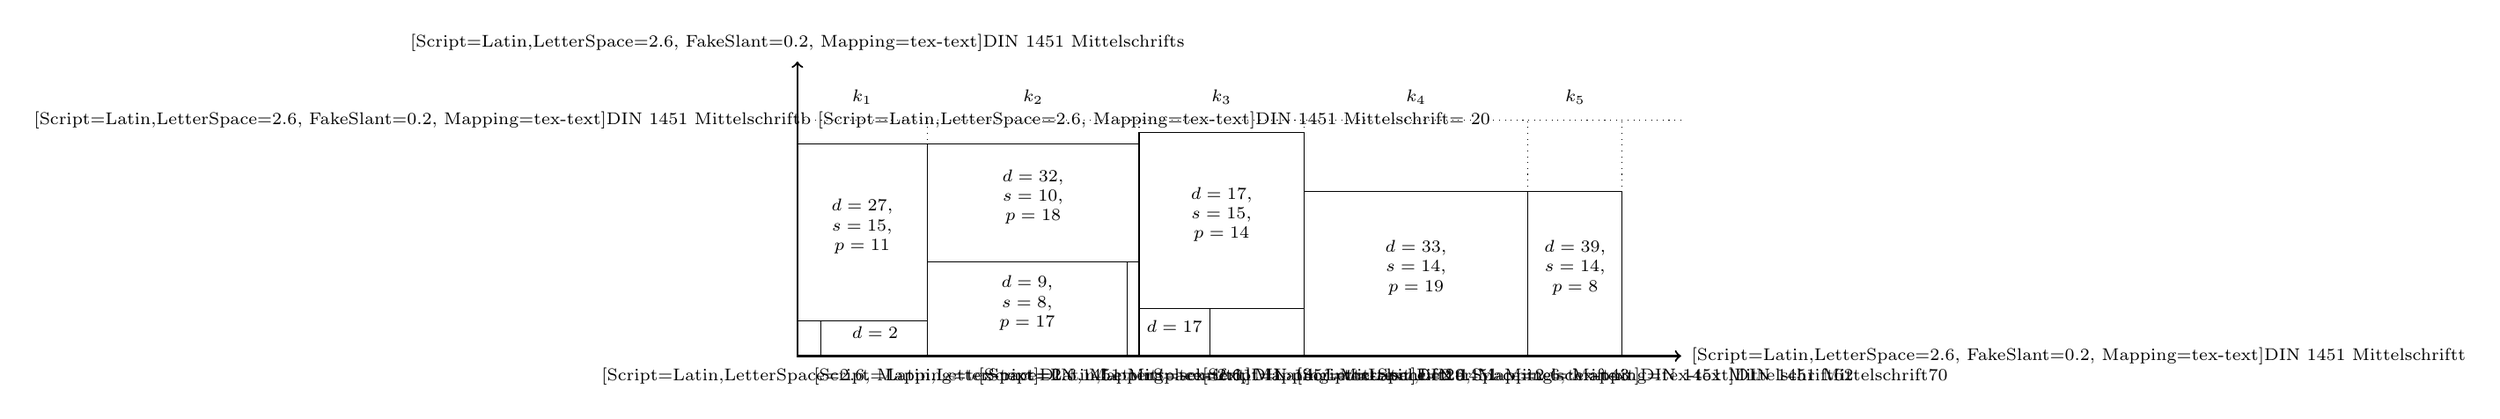
\begin{tikzpicture}[scale=0.17, font=\scriptsize]
      \draw [<->,thick] (0,25) node (yaxis) [above] {\sansitalicfont s}
        |- (75,0) node (xaxis) [right] {\sansitalicfont t};
      \draw[dotted] (0,20) -- (75,20);
      \node at (-3, 20) {{\sansitalicfont b }\sansfont = 20};
        \draw (0,0) rectangle (2,3) node[fn, xshift=2.3em, text width=4em] {$d = 2$};
        \draw (0,3) rectangle (11, 18) node[fn] {$d = 27,$\\ $s=15,$\\ $p = 11$};
        \node at (5.5, 22) {$k_1$};
        \node at (11, -1.7) {\sansfont 11};
      \draw[dotted] (11,0) -- (11,20); 
        \draw (11,0) rectangle (28, 8) node[fn] {$d = 9,$\\ $s=8,$\\ $p=17$};
        \draw (11,8) rectangle (29,18) node[fn] {$d = 32,$\\ $s=10,$\\ $p=18$};
        \node at (20, 22) {$k_2$};
        \node at (29, -1.7) {\sansfont 29};
      \draw[dotted] (29,0) -- (29, 20);
        \draw (29,0) rectangle (35,4) node[fn] {$d = 17$};
        \draw (29,4) rectangle (43,19) node[fn] {$d = 17,$\\ $s=15,$\\ $p=14$};
        \node at (36, 22) {$k_3$};
        \node at (43, -1.7) {\sansfont 43};
      \draw[dotted] (43,0) -- (43, 20);

        \draw (43,0) rectangle (62, 14) node[fn] {$d = 33,$\\ $s=14,$\\ $p=19$};
         \node at (52.5, 22) {$k_4$};
        \node at (62, -1.7) {\sansfont 62};

      \draw[dotted] (62,0) -- (62, 20);
        \draw (62,0) rectangle (70, 14) node[fn] (lastblock) {$d = 39,$\\
        $s=14,$\\ $p=8$};
         \node at (66, 22) {$k_5$};
        \node at (70, -1.7) {\sansfont 70};
      \draw[dotted] (70,0) -- (70, 20);

    \end{tikzpicture}
 \caption{Optimal solution to an example problem with eight
 jobs ($s_j$ and $p_j$ not shown for the two small jobs)}\label{fig:intro_tetris}
\end{figure}

\section{Organization of this paper}
We first provide some background on the fundamental concepts of MIP and CP
(Sections \ref{sec:backgroundmip} and \ref{sec:backgroundcp}), and
review some of the most relevant publications on similar batch scheduling
problems (Section \ref{sec:backgroundlit}) before we describe Malapert's global
constraint in some detail (Section \ref{sec:malapertcp}), as well as his
original MIP model (Section \ref{sec:malapertmip}).

We then present possible improvements to the
model in \ref{sec:improvedmipmodel}. Section \ref{sec:cpmodel} introduces a CP
formulation of the same problem. Sections \ref{sec:mipdecomp} and
\ref{sec:cpdecomp} describe a decomposition approach. Finally, a new MIP approach
is introduced in Section \ref{sec:movebackmip}.

An empirical comparison of the new models and a discussion of the results follow in
Sections \ref{sec:results} and \ref{sec:discussion}. Ideas for future work are
listed in \ref{sec:futurework}.

%%%%%%%%%%%%%%%%%%%%%%%%%%%%%%%%%%%%%%%%%%%%%%%%%%%%%%%%%%%%%%%%%%%%%%
%%%%%%%%%%%%%%%%%%%%%%%%%%%%%%%%%%%%%%%%%%%%%%%%%%%%%%%%%%%%%%%%%%%%%%
%%%%%%%%%%%%%%%%%%%%%%%%%%%%%%%%%%%%%%%%%%%%%%%%%%%%%%%%%%%%%%%%%%%%%%
%%%%%%%%%%%%%%%%%%%%%%% BACKGROUND INFO %%%%%%%%%%%%%%%%%%%%%%%%%%%%%%
%%%%%%%%%%%%%%%%%%%%%%%%%%%%%%%%%%%%%%%%%%%%%%%%%%%%%%%%%%%%%%%%%%%%%%
%%%%%%%%%%%%%%%%%%%%%%%%%%%%%%%%%%%%%%%%%%%%%%%%%%%%%%%%%%%%%%%%%%%%%%
%%%%%%%%%%%%%%%%%%%%%%%%%%%%%%%%%%%%%%%%%%%%%%%%%%%%%%%%%%%%%%%%%%%%%%
%%%%%%%%%%%%%%%%%%%%%%%%%%%%%%%%%%%%%%%%%%%%%%%%%%%%%%%%%%%%%%%%%%%%%%

\chapter{Background}
% citet{Azizoglu} results in [2002]
% citep{Azizoglu} results in [Azizoglu et al., 2002]
% citep*{Azizoglu} results in [Azizoglu and Miller, 2002]
Many optimization problems, and scheduling problems in particular, are
combinatorial in nature. The number of possible solutions grows exponentially
with the number of input variables, and even with fast computers it is
impossible to explore all of them individually to find the best one
(also called ``full enumeration'', or ``brute-force'' search) in a reasonable
amount of time. Often, however, it is possible to reason about subsets of
solutions that are known to be suboptimal a priori. This limits the search
space, allowing us to solve many instances of difficult combinatorial problems
in few hours, minutes or even seconds.

Such constrained searches are often implemented in either one of two ways (or
variants of them): as a \textit{Constraint Programming model} (CP) or as a
\textit{Mixed Integer Programming model} (MIP). In this section I will briefly
introduce the concepts behind both CP and MIP and review recent work on problems
similar to the one dealt with here.

\section{Constraint Programming}
\label{sec:backgroundcp}
Many problems can be understood as situations in which a set of values is to be
chosen according to certain rules, but since the number of possible combinations
of values is enormous, attempting to test all of them is infeasible.


Constraint programming (CP) is a formal framework for the formulation and
solution of such problems. CP models consist of a set of variables $V = \{x_1,
\dots, x_n\}$, each $x_i$ of which has a domain $\mathcal{D}_i$, the set of
values that could conceivably be assigned to it. The CP problem is defined by a
set of relationships that must hold between the variables. Model
\ref{mod:cpsample} illustrates the concept.

\begin{model}
\begin{align}
x &\in \{1,\dots,10\}\\
y &\in \{9,\dots,20\}\\
z &\in \{1,\dots,50\}\\
x &> y\\
z &\geq xy - 42
\end{align}
\caption{A simple CP model}
\label{mod:cpsample}
\end{model}
Here, $x, y, z$ are the variables with their respective domains.

\subsection{Propagation}
We can choose a variable and a value to assign to it, and explore the
consequences of this assignment. Assign $x = 5$, then based on the constraint $x
> y$ only values $< 5$ are permissible for $y$, but none are available in
$\mathcal{D}_y$. The assignment $x = 5$ leads to an \textit{inconsistency}, and
another value must be chosen.
 
If we choose $x = 10$ (which, clearly, is the only feasible value for $x$, since all
others violate $x > y$), $y$ is limited to $y = 9$. This means that $z \geq 9 \cdot
10 - 42 = 48$, thus $z = \{48, 49, 50\}$.
 
This process of successive elimination is known as
\textit{propagation}, and it is the core of all CP solver algorithms. In
propagation, a variable's domain is reduced, and the constraints are used
to reduce the domains of other variables accordingly, until no constraints are
violated.

\subsection{Consistency}
Propagation is commonly seen as a way to enforce consistency. It can be
triggered by fixing a variable to a value, but also by systematic evaluation of
constraints. Let any two variables in a problem be involved in a binary
constraint $C$, such as $x > y$ above. If their domains are such that
they fulfill $C$ (that is, $\forall a \exists b$ such that $a \in
\mathcal{D}_x, b \in \mathcal{D}_y, C(x = a, y = b) = \mathtt{true}$), they are
\textit{arc-consistent} with regards to $C$. Propagation will commonly enforce
arc consistency across all variables and constraints.
 
Arc consistency alone is not sufficient to guarantee the existence of a solution
(satisfiability), unless the graph of variables and constraints is acyclic.
Consider the following problem (Model \ref{mod:unsatcp}):
 
\begin{model}[h!]
\begin{align}
x_1 &= x_2\\
x_1 &= x_3\\
x_2 &= x_4\\
x_3 &\neq x_4\\
x_1, x_2, x_3, x_4 &\in \{1, 2\}
\end{align}
\caption{Unsatisfiable CP problem}
\label{mod:unsatcp}
\end{model}
The model is arc-consistent as given here, but has no solution: forcing any variable to assume
a fixed value will result in at least constraint being violated.
 
The notion of arc consistency (two variables) can be extended, e.g. to three
variables related through binary constraints (\textit{path consistency}) or
to constraints involving more than two variables to \textit{n-consistency} up to
\textit{generalized arc consistency}, where every value assigned to
a variable $x$ must be consistent with all of all other variables' values.

\subsection{Global constraints}
Propagation makes use of graph-theory based algorithms that enforce a form of
consistency on the variables involved in a constraint. Most constraints are
formulated in the form of binary relationships involving a single operator (e.g.
$\geq, =$ or $\neq$). But it is often possible and beneficial to impose
constraints on groups of variables at once. Consider the following classic
example:
\begin{model}[h!]
\begin{align}
x_1 &\neq x_2\\
x_2 &\neq x_3\\
x_3 &\neq x_4\\
x_4 &\neq x_1\\
x_1 &\neq x_3\\
x_2 &\neq x_4\\
x_1, x_2, x_3, x_4 &\in \{1, 2, 3\}
\end{align}
\caption{A clique of not-equal constraints}
\label{mod:cpalldiff}
\end{model}
Model \ref{mod:cpalldiff} prescribes that the variables $x_1, x_2, x_3, x_4$ are
to take on different values. The model is arc-consistent. To find a solution (or
insatisfiability), a value has to be assigned to three of the variables, and the
solver has to propagate the domain reductions after every assignment. Consider,
on the other hand, the use of a specialized constraint called
\texttt{alldifferent}$(x_1, x_2, x_3, x_4)$. This constraint, implemented as a
custom algorithm, can speed up the propagation rapidly. In the case of our
example, the constraint can infer that the number of variables exceeds the
number of available values. The solver can conclude that the problem is
insatisfiable without any propagation.

Such specialized or ``global'' constraints can efficiently exploit properties
that hold for certain relationships among groups of variables, and that would
not be available if the relationship were expressed as a set of binary
constraints.
 
\section{Mixed Integer Programming}
\label{sec:backgroundmip}
\subsection{Linear Programming}
Mixed Integer Programs (or ``MIP
models'') express the minimization of a linear function subject to linear
constraints. If all variables in the problem can be rational in the solution,
the MIP model is really a \textit{linear program} (LP), which can be solved in
polynomial time.\footnote{In practice, variations on Dantzig's \textit{simplex
method} are most often used to solve LPs. Such solvers perform very well on most
problems, but no known variant has been proven to have polynomial worst-case
complexity \citep{papadimitriou}. Solvers with theoretically polynomial-time
complexity exist (Karmarkar's algorithm \citep{karmarkar} has a run-time of
$\mathcal{O}(n^{3.5}L^2 \cdot \log L \cdot \log \log L)$, for instance, where
$L$ is the number of bits of input), but are used less frequently.} This makes
MIP models a generalized and generally more difficult variation on LPs and it is
convenient to introduce them in this order. 

Figure
\begin{figure}
  \centering
    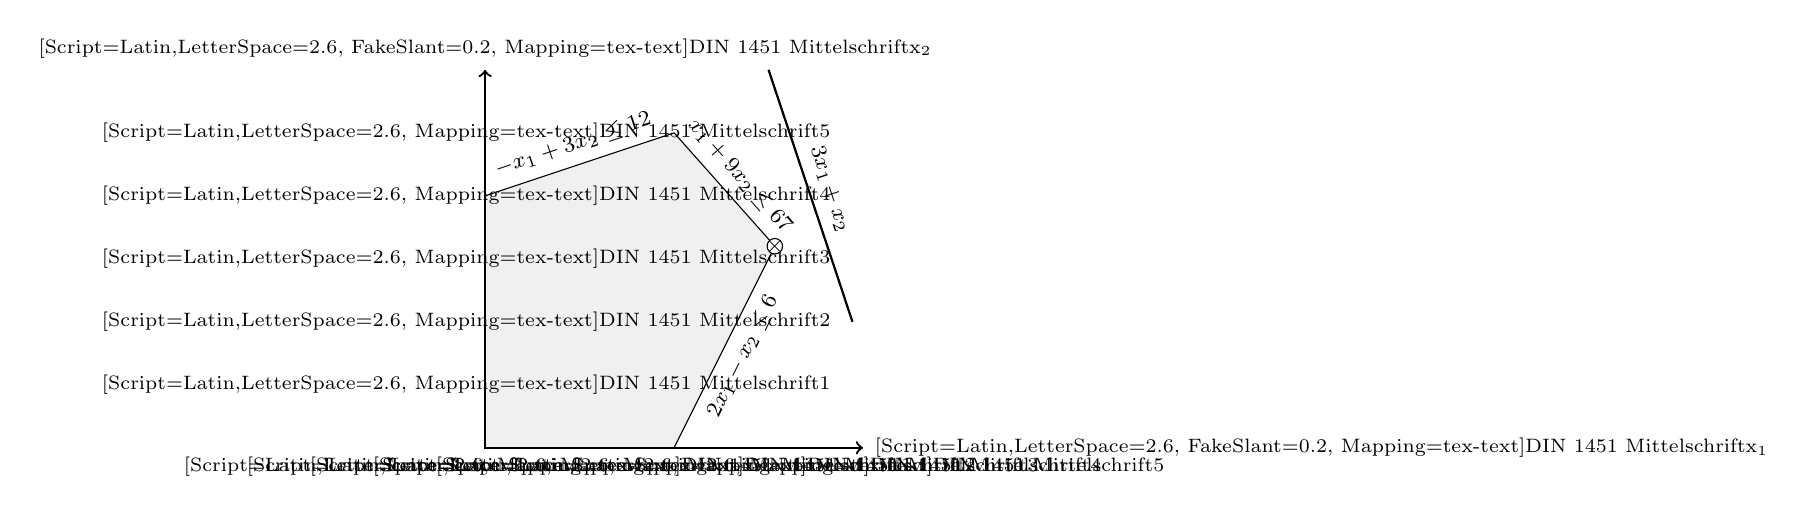
\begin{tikzpicture}[scale=0.8,font=\scriptsize]

      \fill[fill={rgb:black,1;white,16}] (0,0) -- (0,4) -- (3,5) -- (4.6,3.2) -- (3,0) -- cycle;
      \draw [<->,thick] (0,6) node (yaxis) [above] {\sansitalicfont
      x\textsubscript{2}}
        |- (6,0) node (xaxis) [right] {\sansitalicfont x\textsubscript{1}};

      \foreach \x in {1,...,5} \node at (\x,-0.3) {\sansfont \x};
      \foreach \y in {1,...,5} \node at (-0.3, \y) {\sansfont \y};

      \draw (0, 4) -- node[above, sloped] {\footnotesize $-x_1 + 3x_2 \leq 12$} (3,5);
      \draw (3, 0) -- node[below, sloped] {\footnotesize $2x_1 - x_2 \leq 6$}
      (4.6,3.2);
      \draw (3, 5) -- node[above, sloped] {\footnotesize $x_1 + 9x_2 \leq 67$}
      (4.6,3.2);
      
      \draw [thick] (4.5,6) -- node[above, sloped] {\footnotesize $3x_1 + x_2$}
      (5.833,2); 
     
      \draw (4.6,3.2) node[circle,fill=white, inner sep=-0.9pt, draw=black, line 
      width=0.4pt] {\scriptsize$\times$};
    \end{tikzpicture}
 \caption{Graphical representation of a typical LP problem}\label{fig:lpplot1}
 \end{figure}

\ref{fig:lpplot1} illustrates the concept of an LP in two variables, $x_1$ and
$x_2$, as listed in Model \ref{lpintro_model}. The set of feasible solutions is given by the shaded area bounded by the axes
and by three inequalities (``constraints''). A third linear term, the objective
function $3x_1 + x_2$, is to be maximized.\footnote{Minimization is more common,
but note that multiplying the objective by $-1$ achieves this.} 
\begin{model}
\begin{alignat}{2}
\text{Maximize}\quad & 3x_1 + x_2 && \\
\text{subject to the constraints}\quad & -x_1 + 3x_2 \leq 12 &&\\
& x_1 + 9x_2 \leq 67 && \\
& 2x_1 - x_2 \leq 6 && \\
& x_1 \geq 0 && \\
& x_2 \geq 0 && 
\end{alignat}
\caption{A simple LP model, as shown in Figure \ref{fig:lpplot1}}
\label{lpintro_model}
\end{model}

Although the objective function is shown in the figure as a line in a specific
location, note that, as it is not an equation, it can be represented by any line
parallel to that shown in the figure. While we are trying to maximize the
objective value (move the line outwards to the top right), the solution must be
feasible (within the shaded region). It is thus obvious
that the desired extreme value of our objective function is found at one of the
``corners'' of the shaded area: the solution is marked $\otimes$ in the figure.
In fact, since the shaded area generated by linear inequalities will always be a
convex polygon (or polyhedron, in higher dimensions), the solution will
invariably be found at an intersection of hyperplanes.

\subsection{Solving MIP models using branch-and-bound}
MIP models are LPs in which some of the decision variables are declared
integers. Like LP models, MIP models also require an
objective function to be minimized. Figure
\begin{figure}
  \centering
    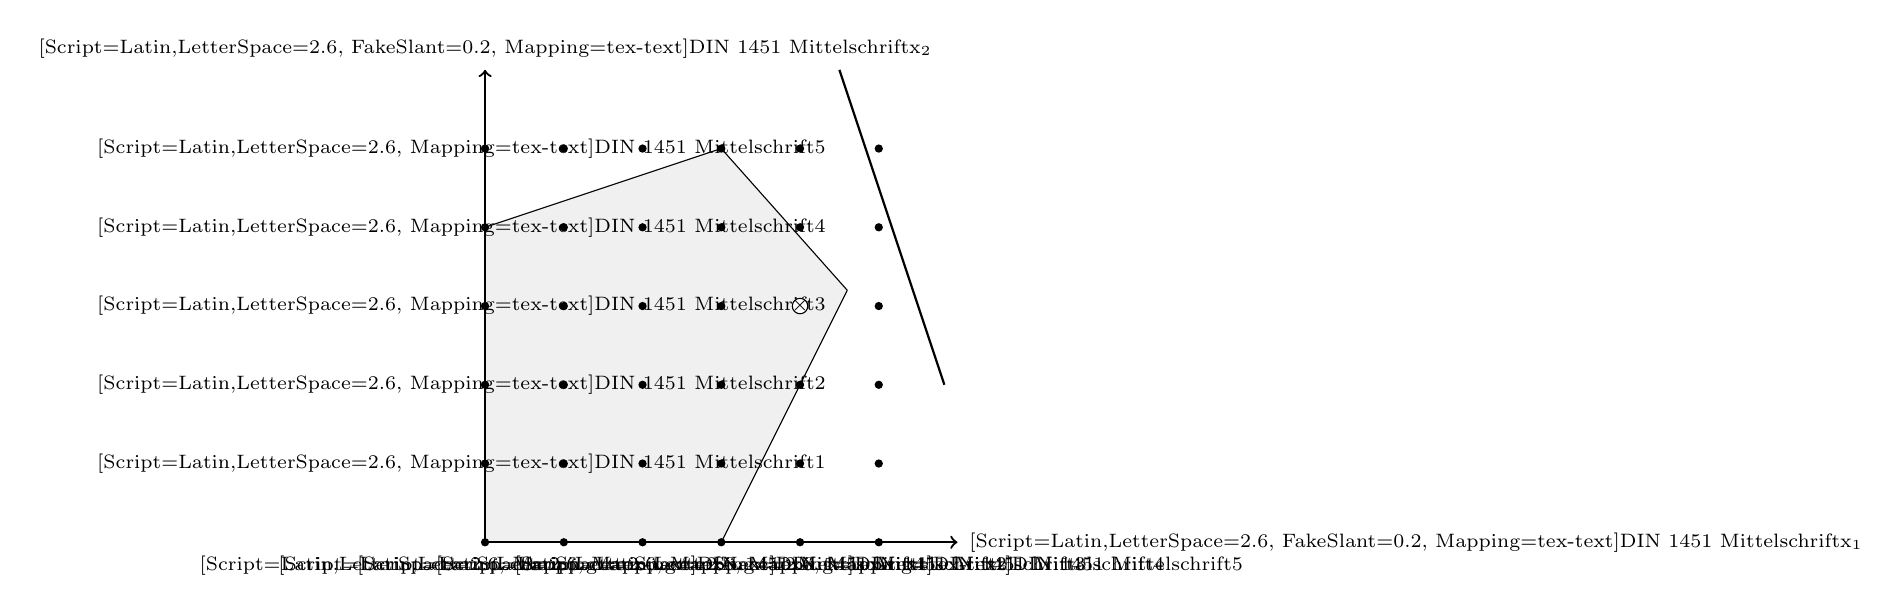
\begin{tikzpicture}[font=\scriptsize]

      \fill[fill={rgb:black,1;white,16}] (0,0) -- (0,4) -- (3,5) -- (4.6,3.2) -- (3,0) -- cycle;
      \draw [<->,thick] (0,6) node (yaxis) [above] {\sansitalicfont
      x\textsubscript{2}}
        |- (6,0) node (xaxis) [right] {\sansitalicfont x\textsubscript{1}};

      \foreach \x in {1,...,5} \node at (\x,-0.3) {\sansfont \x};
      \foreach \y in {1,...,5} \node at (-0.3, \y) {\sansfont \y};

      \draw (0, 4) -- (3,5);
      \draw (3, 0) -- (4.6,3.2);
      \draw (3, 5) -- (4.6,3.2);
      \draw [thick] (4.5,6) -- (5.833,2); 

      \foreach \x in {0,...,5} \foreach \y in {0,...,5}
        \draw (\x, \y) node[circle,fill=black, inner sep=0pt, minimum width=3pt,
        radius=2.5pt] {};
     
      \draw (4,3) node[circle,fill=white, inner sep=-0.9pt, draw=black, line 
      width=0.4pt] {\scriptsize$\times$};
    \end{tikzpicture}
 \caption{Graphical representation of a typical MIP problem}\label{fig:mipplot1}
 \end{figure}

\ref{fig:mipplot1} illustrates this based on the LP problem above: now, only the
black dots represent feasible solutions as both $x_1$ and $x_2$ must be integer. While the solution is easily found in
the figure by inspection (simply round to the nearest feasible integral
solution!), this is not the case in problems with many variables; it is
difficult enough to visualize the problem in three dimensions, and many problems
require hundreds or thousands. Moreover, rounding is particularly unreliable 
with variables of small domains (e.g. binary variables), which are often used in
MIP models to represent decisions. Indeed, solving MIP models is NP-hard.

Similar to CP searches, MIP searches can be thought of as trees, where every
branch represents an assignment of a value to a variable and every leaf represents
a feasible solution. The difference lies in the way MIP explores this search tree.

The MIP solver first solves the problem as an LP, which will usually result in
fractional values for all or most of the variables. In this context, the LP is
known as the \textit{LP relaxation} of the problem---an easier, approximate
version of the original. Assuming we are minimizing the objective, the resulting
LP objective value will be a lower bound on the optimal MIP objective value.
At this point, the solution is $x_1 = 4.6, x_2 = 3.2$.

The solver then chooses a variable, based on heuristics, and \textit{branches}
on it. In this case, assume that we branch on $x_2$, which means that we set
$x_2 \leq 3.0 \lor x_2 \geq 4.0$. We now have two new MIPs, as shown in figure
\ref{fig:mipplot2}. Both of these new subproblems are need solving.\footnote{In
this example, the optimal value for $x_2$ was
within $\pm1$ of its LP value.  This is often the case, and it is not
immediately obvious from the figure why fixing $x_2 = 3.0 \lor x_2 = 4.0$ is
insufficient. In some problems, however, the circumscribed polytope protrudes
relatively far diagonally through the grid of integer solutions, in which case
branching on $\leq \lfloor x_i \rfloor$ and $\geq \lceil x_i \rceil$ is
necessary to capture the optimal feasible solution.} At
this point, another heuristic decides which subproblem is solved first.
Again, the chosen subproblem is first solved in its LP relaxation, and the above
procedure is repeated until an integral solution is found. If this solution is
the best solution known so far, it is stored as the \textit{incumbent}. The
solver then \textit{backtracks}: it undoes some of the previously fixed variables,
and explores other (previously unsolved) subproblems.

This behaviour can be visualized as a search tree in which every node represents
a decision between two subproblems. At every node, a subproblem is chosen, the
subproblem's LP relaxation is run, and the next variable is chosen to be
branched on.

When the solver backtracks to a previous node to explore another subproblem, say
$P_1$, it can compare the LP solution of $P_1$ with the current incumbent's
solution. Since a solution will never improve with additional integrality
constraints, the subtree of $P_1$ can be ignored if the objective value of the
LP solution to $P_1$ is worse than that of the current incumbent. This
``pruning'' of the search tree during the search is referred to as
\textit{bounding}, and is what allows many MIP models to be solved in less time than
their theoretically exponential complexity suggests.

\subsection{Lazy constraints in MIP}\label{sec:lazyconstraints}
Achieving fast search times in MIP requires striking a delicate balance between
keeping the model small (reducing the time needed to solve the LP relaxations)
and formulating the model tightly (pruning more branches off the search tree).
Often, the way certain constraints can be used to perform pre-solve reductions
plays into the performance also, and is difficult to predict.

\textit{Lazy constraints} are one way to avoid this problem. They are expressed
as regular linear constraints and checked against whenever the model encounters
a new solution. Lazy constraints that were violated are then added to the model
to be used in future instances.

This is particularly useful when a problem lends itself to the generation of
vast sets of constraints involving few variables, but most of these constraints
are likely not needed. In such cases, lazy constraints can greatly speed up
solution times.

\section{Scheduling using CP and MIP}
\subsection{Common characteristics of scheduling problems}
Many scheduling problems can be described by some of the following
characteristics:
\begin{description}
\item[Objective]{In this paper, $\Lmax$ is the value to be minimized. Other
situations might call for minimization of the makespan ($C_\text{max}$), the
maximum tardiness (like lateness, but never below zero), total completion time
weighed differently for every job, or other measures.}
\item[Number of resources]{Some problems, like the one treated in this paper,
assume the existence of only one resource. Other problems, e.g. \textit{flow
shop} or \textit{open shop} problems, require multiple resources.}
\item[Release dates and precedence constraints]{Many problems specify that
certain jobs must finish before other jobs begin, and/or that they may not start
before a certain time.}
\item[Resource type]{In this paper, the resource processes batches only. Other
resources may be \textit{disjunctive}, allowing execution of one job at a time
only, or \textit{cumulative}, allowing for multiple jobs to be processed in
parallel without any batching restriction. \textit{Pre-emptive} processing means
that jobs may be interrupted and continued at a later time, which greatly
improves the flexibility and, in turn, the objective value of the resulting
schedule.}
\end{description}

Scheduling problems are commonly summarized as an abbreviated expression
summarizing the above and other properties in a format introduced by
\citet{graham}. For the problem at hand, it is $1|\textit{p-batch}; b < n;
\textit{non-identical}|\Lmax$.

\subsection{Scheduling problems in CP}
\label{sec:schedulingcp}
CP solvers work by reducing the domains of variables, and so it is only natural
to express the position of a job using variables such as $\mathtt{startOf}(j)$
or $\mathtt{endOf}(j)$, the domains of which are then reduced to feasible
values. This creates the notion of an earliest/latest start/finish time of a job,
commonly abbreviated \texttt{est}/\texttt{lst}/\texttt{eft}/\texttt{lft}.

The most well-known propagation techniques on these four variable bounds are
called \textit{edge finding}: they reason about a job's time bounds and whether
they allow it (or force it) to execute before or after a set of other jobs on
the same resource.

Capacity constraints are often expressed as \texttt{cumulative} and/or
\texttt{pack} global constraints, efficient (and problem-agnostic)
implementations of which are part of every major CP software package.

\subsection{Scheduling problems in MIP}
The position of a job in time is more difficult to represent in MIP
formulations. Most models can roughly be divided into two groups:

\paragraph{Time-indexed/discrete-time formulations.} In this type of model, a set of binary
variables is used to indicate the start time (or end time) of a job on a
predefined, discrete grid of time points. The binary variables must sum to one.
Capacity constraints (e.g. cumulative constraints) can then be imposed by means
of relationships between start times of pairs of jobs, their sizes and
processing times. This kind of model is be relatively easy to extend and work
with, but the number of variables and constraints required grows (at least) with
the square of the number of jobs involved.

\paragraph{Disjunctive/continuous-time formulations.}
In this type of model, jobs' start times are represented by single variables,
and for a pair of jobs, the difference between their start times must exceed the
earlier-scheduled job's processing time on a disjunctive resource.

\section{Literature Review}
\label{sec:backgroundlit}
An extensive and application-based introduction to MIP models is given by
\citet{williams}. \citet{bartak} presents a detailed survey of common constraint
programming techniques. \citet{pinedo} gives a comprehensive overview over
topics and algorithms in artificial scheduling.

The problem at hand is based on the work of \citet{Malapert}, who proposed a global
constraint \texttt{sequenceEDD} to be used in combination with \texttt{pack} to
solve it to optimality. The \texttt{sequenceEDD} constraint is implemented as
four distinct filtering rules applied at relevant domain changes: three to update
bounds on $\Lmax$ based on different conditions, and one to limit the number of
batches based on the marginal cost difference between adding a job to an empty
batch vs. an existing one. The new global was shown to significantly outperform
a simple MIP model of the same problem, as well as a branch-and-price model
proposed by \citet{Daste1}.

Other authors have examined similar problems: \citet{Azizoglu} provide an exact
method and a heuristic for the same problem, but minimize makespan
($C_\text{max}$) instead of $\Lmax$, as have \citet{Dupont}. Similar exact
methods have been proposed for multi-agent variants with different objective
functions \citep{Sabouni}, for makespan minimization on single batch machines
\citep{Kashan}, and for makespan minimization on parallel batch machines with
different release dates \citep{Ozturk}. A more extensive review of MIP model
applications in batch processing is given by \citet{Grossmann}.


%%%%%%%%%%%%%%%%%%%%%%%%%%%%%%%%%%%%%%%%%%%%%%%%%%%%%%%%%%%%%%%%%%%%%%
%%%%%%%%%%%%%%%%%%%%%%%%%%%%%%%%%%%%%%%%%%%%%%%%%%%%%%%%%%%%%%%%%%%%%%
%%%%%%%%%%%%%%%%%%%%%%%%%%%%%%%%%%%%%%%%%%%%%%%%%%%%%%%%%%%%%%%%%%%%%%
%%%%%%%%%%%%%%%%%%%%%%% MALAPERT'S MODELS %%%%%%%%%%%%%%%%%%%%%%%%%%%%
%%%%%%%%%%%%%%%%%%%%%%%%%%%%%%%%%%%%%%%%%%%%%%%%%%%%%%%%%%%%%%%%%%%%%%
%%%%%%%%%%%%%%%%%%%%%%%%%%%%%%%%%%%%%%%%%%%%%%%%%%%%%%%%%%%%%%%%%%%%%%
%%%%%%%%%%%%%%%%%%%%%%%%%%%%%%%%%%%%%%%%%%%%%%%%%%%%%%%%%%%%%%%%%%%%%%
%%%%%%%%%%%%%%%%%%%%%%%%%%%%%%%%%%%%%%%%%%%%%%%%%%%%%%%%%%%%%%%%%%%%%%
\chapter[State of the Art: Recent work by Malapert]{State of the Art:\\ Recent work by Malapert}
\label{sec:malapertcp}
\section{The sequenceEDD global constraint}
In their 2011 paper, Malapert et al. present a CP formulation of the problem
which, in essence, relies on two global constraints: \texttt{pack}, which
constraints job-to-batch assignments such that no capacity limits are violated,
and \texttt{sequenceEDD}, which sorts batches into EDD order. The implementation
of the latter constraint includes a set of rules which update the current
$\Lmax$, lower and upper bounds on $\Lmax$, and lower and upper bounds on the
number of batches in the optimal solution every time \texttt{sequenceEDD} is
triggered by a job-batch assignment. Based on these bounds, other assignments
are then eliminated from the set of feasible assignments.

\subsection{Filtering rules}
\paragraph{\textit{Final lateness filtering rule} and \textit{lateness filtering
rule.}} The algorithm calculates the value
of $\Lmax$ given a partial assignment $\mathcal{A}$. This value is also a lower
bound on the $\Lmax$ of any assignment $\mathcal{A}'$ extending $\mathcal{A}$,
since assigning more jobs to batches will never improve $\Lmax$.\footnote{An
\textit{assignment} $\mathcal{A}$ in this context refers to a set of
job-to-batch assignments for any subset of jobs $J_\mathcal{A} \subseteq J$. A
given assignment $\mathcal{A}$ can be \textit{extended} to $\mathcal{A}'$ by
assigning one or more additional (i.e.  previously unassigned) jobs to batches.}

\paragraph{\textit{Cost-based domain filtering rule of assignments.}} This rule
eliminates possible assignments of yet-unassigned jobs $j$ to batches $k$, if
such assignments cause $\Lmax$ to exceed the current known upper bound on
$\Lmax$ (or best known solution).

\paragraph{\textit{Cost-based domain filtering based on bin packing.}} The
following set of rules considers the number of non-empty batches $M$ used in the
final solution. First, lower and upper bounds on $M$ are updated based on the
number of batches currently in use and on the number of unassigned (``open'')
jobs. Then, the set of shortest remaining jobs is used to update to compute a
lower bound on $\Lmax$ given a hypothetical solution using exactly $M = m$
non-empty batches. Based on this lower bound, the current lower bound on
$\Lmax$ is updated. Finally, the upper bound on $M$ is decremented until the
lower bound on $\Lmax$ given $M$ batches no longer exceeds the current upper
bound on $\Lmax$.

These four filtering rules serve to systematically reduce the solution space as
the search progresses.

\subsection{Search heuristic}
\label{sec:bestfit}
The search heuristic chosen for the packing of a job $j$ into a set of batches
$K$ is to prefer assignment to batch $k$ having the lowest value of $\gamma(B_j
\leftarrow k)$, approximating the fitness of $j$ into $k$ given the current
assignment $\mathcal{A}$:
\begin{align}
\gamma(B_j \leftarrow k) = \frac{ |\min(P_k) - p_j| }{\underset{J}{\max}(p_j) -
\underset{J}{\min}(p_j)} + \frac{ |\max(D_k) - d_j| }{\underset{J}{\max}(d_j) -
\underset{J}{\min}(d_j)}
\end{align}

We reference this heuristic in Section \ref{sec:ublmax}, where we use it to
determine an initial upper bound on the value of $\Lmax$.

\section{MIP formulation}
\label{sec:malapertmip}
Malapert's original MIP formulation is given in Model \ref{model:malapertmip}. It
uses a set of binary decision variables $x_{jk}$ to represent whether job $j$ is
assigned to batch $k$. The original model assumes a set $K$ of $|K| = |J|$
batches, the number of jobs being a trivial upper bound on the number of batches
required; it also enforces an earliest-due-date-first (EDD) ordering of the
batches (constraint \eqref{c:malapp-edd}).

\begin{model}[h]
\begin{alignat}{2}
\mathrm{Min.}\quad & \Lmax && \\
\mathrm{s.t.}\quad &\sum_{k \in K} x_{jk} = 1 \quad && \forall j \in J
\label{c:malapp-unique}\\
  &\sum_{j \in J} s_j x_{jk} \leq b \quad && \forall k \in K\label{c:malapp-cap}\\
  &p_j x_{jk} \leq P_k \quad && \forall j \in J, \forall k \in
  K\label{c:malapp-pk}\\
  &C_{k-1} + P_{k} = C_k \quad && \forall k \in K\label{c:malapp-ck}\\
  &(d_{max} - d_j)(1 - x_{jk}) + d_j \geq D_k \quad && \forall j \in J, \forall
  k \in K\label{c:malapp-dk}\\
  &D_{k-1} \leq D_k \quad && \forall k \in K \label{c:malapp-edd} \\
  &C_k - D_k \leq \Lmax \quad && \forall k \in K\label{c:malapp-lmax}\\[2ex]
  &C_k \geq 0, P_k \geq 0 \text{ and } D_k \geq 0 \quad && \forall k \in K  
\end{alignat}
\caption{Malapert's original MIP model}
\label{model:malapertmip}
\end{model}

Constraints \eqref{c:malapp-unique} ensure that every job $j$ is assigned to
one batch $k$, and one batch only. Constraints \eqref{c:malapp-cap} ensure that
no batch exceeds the machine's capacity $b$. Constraints \eqref{c:malapp-pk}
define each batch's processing time $P_k$ as the maximum processing time of the
jobs $j$ assigned to it. Constraints \eqref{c:malapp-ck} define each batch's
completion time $C_k$ as that of the previous batch, plus the previous batch's
processing time. Constraints \eqref{c:malapp-edd} ensure that batches are
ordered by due date. Constraints \eqref{c:malapp-lmax} define the objective
value $\Lmax$.

%%%%%%%%%%%%%%%%%%%%%%%%%%%%%%%%%%%%%%%%%%%%%%%%%%%%%%%%%%%%%%%%%%%%%%
%%%%%%%%%%%%%%%%%%%%%%%%%%%%%%%%%%%%%%%%%%%%%%%%%%%%%%%%%%%%%%%%%%%%%%
%%%%%%%%%%%%%%%%%%%%%%%%%%%%%%%%%%%%%%%%%%%%%%%%%%%%%%%%%%%%%%%%%%%%%%
%%%%%%%%%%%%%%%%%%%%%%% MY CONTRIBUTIONS %%%%%%%%%%%%%%%%%%%%%%%%%%%%%
%%%%%%%%%%%%%%%%%%%%%%%%%%%%%%%%%%%%%%%%%%%%%%%%%%%%%%%%%%%%%%%%%%%%%%
%%%%%%%%%%%%%%%%%%%%%%%%%%%%%%%%%%%%%%%%%%%%%%%%%%%%%%%%%%%%%%%%%%%%%%
%%%%%%%%%%%%%%%%%%%%%%%%%%%%%%%%%%%%%%%%%%%%%%%%%%%%%%%%%%%%%%%%%%%%%%
%%%%%%%%%%%%%%%%%%%%%%%%%%%%%%%%%%%%%%%%%%%%%%%%%%%%%%%%%%%%%%%%%%%%%%

\chapter{Modelling the problem} 
In this section we present the models examined.
Beginning with the MIP model used by Malapert, we explore several additional
constraints that, while redundant, tighten the search space. We comment on the
performance of the approaches (see Section \ref{sec:results} for a
comprehensive comparison of performance). We present a CP model and a
decomposition-based approach using either MIP or CP. Finally, we introduce a new
approach to setting up a MIP model that significantly improves upon the original
MIP and outperforms all other models presented in this paper.

All MIP and CP models were implemented in C++ using IBM Ilog's Cplex and CP
Optimizer solvers, respectively.

\section{MIP model}\label{sec:malapertmipmodel}
We first replicated Malapert's original MIP approach, as given in Model
\ref{model:malapertmip}, to establish a performance baseline to compare other
models to. The original model assumes a
set $K$ of $|K| = |J|$ batches, the number of jobs being a trivial upper bound
on the number of batches required; it also enforces an earliest-due-date-first
(EDD) ordering of the batches (constraint \eqref{c:malapp-edd} in Model
\ref{model:malapertmip}).

\section{Improved MIP model}\label{sec:improvedmipmodel}
Several improvements can be made to Malapert's MIP model in the form of
additional constraints shown in Model \ref{model:improvedmip}, as  
described in greater detail in the subsections below.

\begin{model}[h]
\begin{alignat}{2}
& \sum_{j \in J} x_{j,k-1} = 0 \rightarrow \sum_{j \in J} x_{jk} = 0 \quad &&
\forall k \in K \\
& e_k + \sum_{j \in J} x_{jk} \geq 1 \quad && \forall k \in K \\
& n_j (e_k-1) + \sum_{j \in J} x_{jk} \leq 0 \quad && \forall k \in K \\
& e_k - e_{k-1} \geq 0 \quad && \forall k \in K \\
& x_{jk} = 0 \quad && \forall \{j \in J, k \in K | j > k \} \\
& \Lmax \geq \big\lceil\frac{1}{b} \sum_{j} s_j
p_j\big\rceil - \delta_q \quad
&& \forall q, \forall \{ j \in J | d_j \leq \delta_q \}
\end{alignat}
\caption{Improvements to Malapert's original MIP model}
\label{model:improvedmip}
\end{model}

\subsection{Grouping empty batches} The given
formulation lacks a rule that ensures that no empty batch is followed by a
non-empty batch. Empty batches have no processing time and a due date only
bounded by $d_\text{max}$, so they can be sequenced between non-empty batches
without negatively affecting $\Lmax$. Since, however, desirable schedules have
no empty batches scattered throughout, we can easily reduce the search space by
disallowing such arrangements. The idea is illustrated in Figure
\ref{fig:dominancerule}.


\begin{figure}
  \centering
  \begin{subfigure}[b]{0.4\textwidth}
    \centering
    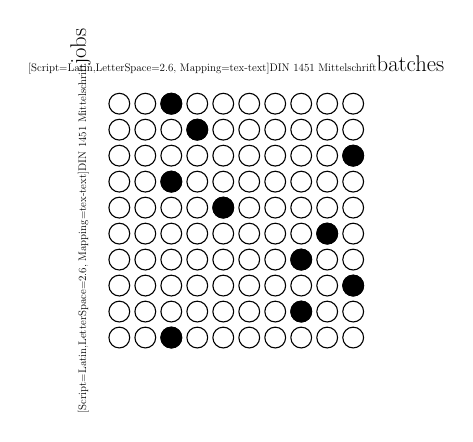
\begin{tikzpicture}[scale=0.33]
      \pgftext[x=-1.5cm, y=4.5cm, rotate=90]{\sansfont\Huge jobs}
      \pgftext[x=4.5cm, y=10.5cm]{\sansfont\Huge batches}

      \foreach \j in {0,...,9}
      {
        \foreach \k in {0,...,9}
        {
          \draw[] (\k, \j) circle [radius=0.4];
        }
      }
      \draw [fill] (2,0) circle [radius=0.4];
      \draw [fill] (2,6) circle [radius=0.4];
      \draw [fill] (2,9) circle [radius=0.4];
      \draw [fill] (3,8) circle [radius=0.4];
      \draw [fill] (4,5) circle [radius=0.4];
      \draw [fill] (7,1) circle [radius=0.4];
      \draw [fill] (7,3) circle [radius=0.4];
      \draw [fill] (8,4) circle [radius=0.4];
      \draw [fill] (9,2) circle [radius=0.4];
      \draw [fill] (9,7) circle [radius=0.4];
    \end{tikzpicture}
    \caption{Without dominance rule}
  \end{subfigure}
  \begin{subfigure}[b]{0.4\textwidth}
    \centering
    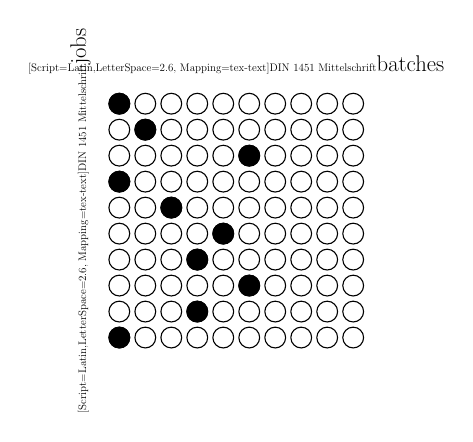
\begin{tikzpicture}[scale=0.33]
      \pgftext[x=-1.5cm, y=4.5cm, rotate=90]{\sansfont\Huge jobs}
      \pgftext[x=4.5cm, y=10.5cm]{\sansfont\Huge batches}

      \foreach \j in {0,...,9}
      {
        \foreach \k in {0,...,9}
        {
          \draw[] (\k, \j) circle [radius=0.4];
        }
      }
      \draw [fill] (0,0) circle [radius=0.4];
      \draw [fill] (0,6) circle [radius=0.4];
      \draw [fill] (0,9) circle [radius=0.4];
      \draw [fill] (1,8) circle [radius=0.4];
      \draw [fill] (2,5) circle [radius=0.4];
      \draw [fill] (3,1) circle [radius=0.4];
      \draw [fill] (3,3) circle [radius=0.4];
      \draw [fill] (4,4) circle [radius=0.4];
      \draw [fill] (5,2) circle [radius=0.4];
      \draw [fill] (5,7) circle [radius=0.4];
    \end{tikzpicture}
    \caption{With dominance rule}
  \end{subfigure}
\caption{Dominance rule to eliminate empty batches followed by non-empty batches
(circles represent the $x_{jk}$ variables; a filled circle stands for $x_{jk} =
1$)}\label{fig:dominancerule}
\end{figure}


A mathematical formulation is
\begin{alignat}{2}
& \sum_{j \in J} x_{j,k-1} = 0 \rightarrow \sum_{j \in J} x_{jk} = 0 \quad && \forall k \in K. \label{eq:emptybatch0}
\end{alignat}

To implement this, we can write constraints in terms of an additional  set of binary variables, $e_k$, indicating whether a batch $k$ is empty or not:
\begin{alignat}{2}
& e_k + \sum_{j \in J} x_{jk} \geq 1 \quad && \forall k \in K, \label{eq:emptybatch1} \\
& n_j (e_k-1) + \sum_{j \in J} x_{jk} \leq 0 \quad && \forall k \in K. \label{eq:emptybatch2}
\end{alignat}

Constraints \eqref{eq:emptybatch1} enforce $e_k = 1$ when the batch $k$ is
empty. Constraints \eqref{eq:emptybatch2} enforce $e_k = 0$ otherwise, since the
sum term will never exceed the number of jobs $n_j$. The rule \eqref{eq:emptybatch0} can now be
expressed as $e_{k-1} = 1 \rightarrow e_k = 1$, and implemented as follows:
\begin{alignat}{2}
& e_k - e_{k-1} \geq 0 \quad && \forall k \in K.
\end{alignat}

We can also prune any attempts to leave the first batch empty by adding a constraint $e_0 = 0$.

\subsection{No postponing of jobs to later batches}
\label{sec:nopostponing}
Consider a schedule in which all jobs are assigned to a single batch (i.e.
$x_{jk} = 1 \forall j = k$), ordered by non-decreasing due date, and by
non-decreasing processing time in case of a tie between two jobs. For the
purposes of this paper, we refer to this schedule as the \textit{single-EDD}
schedule. 

Since, as shown above, there exists an optimal solution with EDD-ordered
batches, we can restrict the search to such solutions. Any solution in which
a job $j$ is moved into a batch $h$ later than its single-EDD batch $k$, i.e. $h
> j = k$, necessarily results in a non-EDD solution. We can therefore write
\begin{alignat}{2}
  & x_{jk} = 0 \quad && \forall \{j \in J, k \in K | j > k \} \label{eq:mipnopp}
\end{alignat}

to exclude solutions in which jobs are assigned to later batches than their
respective single-EDD batch.
%%%% TODO: Explain why the shorter one needs to come first.

\subsection[Lower bound on $\Lmax$]{Lower bound on {\sansitalicfont L}\textsubscript{max}}
Let a \textit{bucket} $q$ denote the set of all batches with due date
$\delta_q$, as defined by \citet{Malapert}.
Then the completion date $C_q$ of this bucket is the completion date of the
last-scheduled batch with due date $\delta_q$, and the lateness of the bucket
$q$ is $L_q = C_q - \delta_q$. Since all batches up to and including those in
bucket $q$ are guaranteed to contain all jobs with due dates $d \leq \delta_q$,
as ensured by the EDD ordering of batches, the lower bound on every bucket's
lateness $LB(L_q)$ is a valid lower bound on $\Lmax$. In other words,
jobs with due date $d \leq \delta_q$ will be found only in batches up to and
including the last
batch of bucket $q$. This provides a lower bound on the lateness of bucket $q$:
\begin{alignat}{2}
& \Lmax \geq C_{\text{max},q} - \delta_q \quad && \forall q
\end{alignat}
The buckets up to bucket $q$ will likely also contain some later-due ($d >
\delta_q$) jobs in the optimal solution, which weakens $LB(L_q)$'s usefulness
but does not affect its validity as a lower bound.

Now we need to find $C_{\text{max},q}$, or at least a lower bound on it, in
polynomial time. The simplest approach simply considers the jobs' total ``area''
(or ``energy''), i.e. the sum of all $s_j p_j$ products:
\begin{alignat}{2}
& C_{\text{max},q} \geq \big\lceil\frac{1}{b} \sum_{j} s_j
p_j\big\rceil \quad
&& \forall q, \forall \{ j \in J | d_j \leq \delta_q \}
\end{alignat}
A better lower bound on $C_{\text{max},q}$ would be given by a
preemptive-cumulative schedule. Unfortunately, minimizing $C_{\text{max}}$ for
such problems is equivalent to solving a standard bin-packing problem, which
requires exponential time.\footnote{In a preemptive-cumulative schedule, jobs
may be stopped and restarted mid-execution, but occupy a constant amount $s_j$
on the resource while executing. In such a schedule, minimizing the makespan is
as difficult as solving a bin-packing problem: we can break jobs into small
pieces (no longer than the smallest common divisor of the jobs' lengths $p$) and
then pack them together such as to minimize the number of small time slots
needed.}

\section{CP model}\label{sec:cpmodel}
The constraint programming model is based on a set of decision variables $B_j
\in \{k_1, \dots, k_{n_k} \}$, where each variable $B_j$ stands for the batch job $j$ is
assigned to. The complete model is given in Model \ref{model:cpmodel}.
\begin{model}
\begin{alignat}{2}
\mathrm{Min.}\quad & \Lmax && \\
\mathrm{s.t.}\quad & \label{cpcs:pack} \mathtt{pack}(J, K, b) && \\
& \label{cpcs:cumul} \mathtt{cumul}(J, b) && \\
& \label{cpcs:pk} P_k = \underset{j}{\max} \; p_j \quad && \forall \{j \in J
| B_j = k\}, \forall k \in K \\
& \label{cpcs:dk} D_k = \underset{j}{\min} \; d_j \quad && \forall \{j \in J
| B_j = k\}, \forall k \in K \\
& \label{cpcs:ck} C_k + P_{k+1} = C_{k+1} \quad && \forall k \in K \\
& \label{cpcs:lmax} \Lmax \geq \underset{k}{\max} \; (C_k - D_k) && \\
& \label{cpcs:empty} \mathtt{IfThen}(P_k = 0, P_{k+1} = 0) \quad && \forall k
\in \{ k_1, \dots, k_{n_k - 2}\} \\
& \label{cpcs:pp} B_j \leq k \quad && \forall \{ j \in J, k \in K | j > k \}
\end{alignat}
\caption{Constraint programming model}
\label{model:cpmodel}
\end{model}

Constraint \eqref{cpcs:pack} makes sure the jobs are distributed into the
batches such that no batch exceeds the capacity $b$. Constraint
\eqref{cpcs:cumul}, a global cumulative constraint, keeps jobs from overlapping
on the resource---while redundant with \eqref{cpcs:pack}, this speeds up
propagation slightly. Constraints \eqref{cpcs:pk}, \eqref{cpcs:dk},
\eqref{cpcs:ck} and \eqref{cpcs:lmax} define $P_k$, $D_k$, $C_k$ (batch
completion time) and $\Lmax$, respectively.

\begin{comment}
\subsection{Temporal constraints on a job's start date} Given any partial
assignment of jobs and an open job $j$, we can reason that \begin{alist}
\item{if the first batch with a due date later than the job is $k$, then the job
cannot be part of a batch after $k$---this would result in a non-EDD sequence
of batches.} \item{if the first batches up to $k-1$ offer not enough capacity
for $j$ due to the given partial assignment, then the job cannot be part of a
batch before $k$.} \end{alist} Since batches are \textit{not} dynamically
created like in Malapert's solution but fixed from the start, any partial
assignment that fails due to these constraints cannot be part of an optimal
solution.

This constraint is redundant with both the $(C_{k+1}\geq C_k)$ and
\texttt{packing} constraints, but may help accelerate the propagation in some
cases.
\end{comment}

\subsection{Grouping empty batches} We can force
empty batches to the back of the schedule and thus establish dominance of
certain solutions. The implementation is much easier than in the MIP model: 
\begin{alignat}{2} &
\mathtt{IfThen}( P_k = 0, P_{k+1} = 0 ) \quad && \forall k \in
\{k_1, \dots, k_{n_k-1}\}
\end{alignat}

\subsection{No postponing of jobs to later batches} Just like in the MIP model,
jobs should never go into a batch with an index greater than their own:
\begin{alignat}{2}
& B_j \leq k \quad && \forall \{j \in J, k \in K | j > k \}
\end{alignat}

\section{Decomposition approach}
Instead of solving the entire problem using a single model, we can solve the
problem step by step, using the best techniques available for each subproblem.
This approach is inspired by \textit{Benders decomposition}.

\label{sec:mipdecomp}
A basic version of this approach uses branch-and-bound to traverse the search
tree. At each node on level $\ell$, a single MIP and/or CP model is run to
assign jobs to batch $k = \ell$. The remaining jobs are passed to the children
nodes, which assign jobs to the next batch, and so on---until a solution, and
thus a new upper bound on $\Lmax$, is found. Several constraints are used to
prune parts of the search tree that are known to offer only solutions worse than
this upper bound. Figure \ref{fig:decomp_diagram1} shows an example in which a
MIP model is used to assign jobs to the batch at every node.
\begin{algorithm}[h]
\fontsize{9pt}{11.5pt}\selectfont
\begin{algorithmic}
\State update \textit{currentAssignments} \Comment{this keeps track of where we are
in the tree}
\If{no jobs given to this node} \Comment{if this is a leaf node, i.e. all jobs
are assigned to batches}
  \State calculate $L_{\text{max,current}}$ based on \textit{currentAssignments}
  \If{$L_{\text{max,current}}$ < $L_{\text{max,incumbent}}$}
    \State $L_{\text{max,incumbent}} \gets L_{\text{max,current}}$
    \State \textit{bestAssignments} $\gets$ \textit{currentAssignments}
  \EndIf
  \State return to parent node
\EndIf
\State set up MIP model \Comment{as described below}
\Repeat
  \State $x_j \gets$ model.solve($x_j$) \Comment{let model assign jobs to the
  batch}
  \State spawn and run child node with all $\{j | x_j = 0\}$ \Comment{pass
  unassigned jobs to children}
  \State add constraint to keep this solution from recurring \Comment{this
  happens once the child node returns}
\Until{model has no more solutions}
\State return to parent node
\end{algorithmic}
\caption{MIP node class code overview}
\label{alg:bbnode_mip1}
\end{algorithm}
Algorithm \ref{alg:bbnode_mip1} outlines what happens at each node: the model
finds the best jobs to assign to the batch according to some rule, lets the
children handle the remaining jobs, and tries the next best solution once the
first child has explored its subtree and backtracked.
\subsubsection{Using MIP and cumulative packing after the batch}
\tikzset{
  treenode/.style = {align=center, inner sep=4pt, text centered,
    font=\sansfont\fontsize{11pt}{12pt}\selectfont},
  root/.style = {treenode},% arbre rouge noir, noeud noir
  nchild/.style = {treenode,
     },% arbre rouge noir, noeud rouge
  leaf/.style = {treenode}% arbre rouge noir, nil
}

\begin{figure}
\centering
\begin{tikzpicture}[->,>=stealth',level/.style={sibling distance = 3cm/#1,
  level distance = 1.5cm}, scale=0.7]
\node (Root) [root] {MIP}
 child{ node [nchild] {MIP} 
            child{ node [nchild] {MIP}}
            child{ node [nchild] {MIP}
              child{ node [leaf] {Solution 1}}
						}                            
    }
    child{ node [nchild] {MIP} }
    child{ node [nchild] {MIP} 
            child{ node [nchild] {MIP} %2, left
                    child{ node [leaf] {Solution 2}} 
                  }
            child{ node [nchild] {MIP} }
		};
  \begin{scope}[every node/.style={right}]
    \path (Root -| Root-3-2) ++(1.5cm,0) node {\fontsize{10pt}{10pt}\selectfont $k=1$};
    \path (Root-1 -| Root-3-2) ++(1.5cm,0) node
    {\fontsize{10pt}{10pt}\selectfont $k=2$};
    \path (Root-1-1 -| Root-3-2) ++(1.5cm,0) node
    {\fontsize{10pt}{10pt}\selectfont $k=3$};
  \end{scope}

   \end{tikzpicture}
\caption{Batch-by-batch decomposition using MIP only}\label{fig:decomp_diagram1}
\end{figure}

\begin{figure}
  \centering
    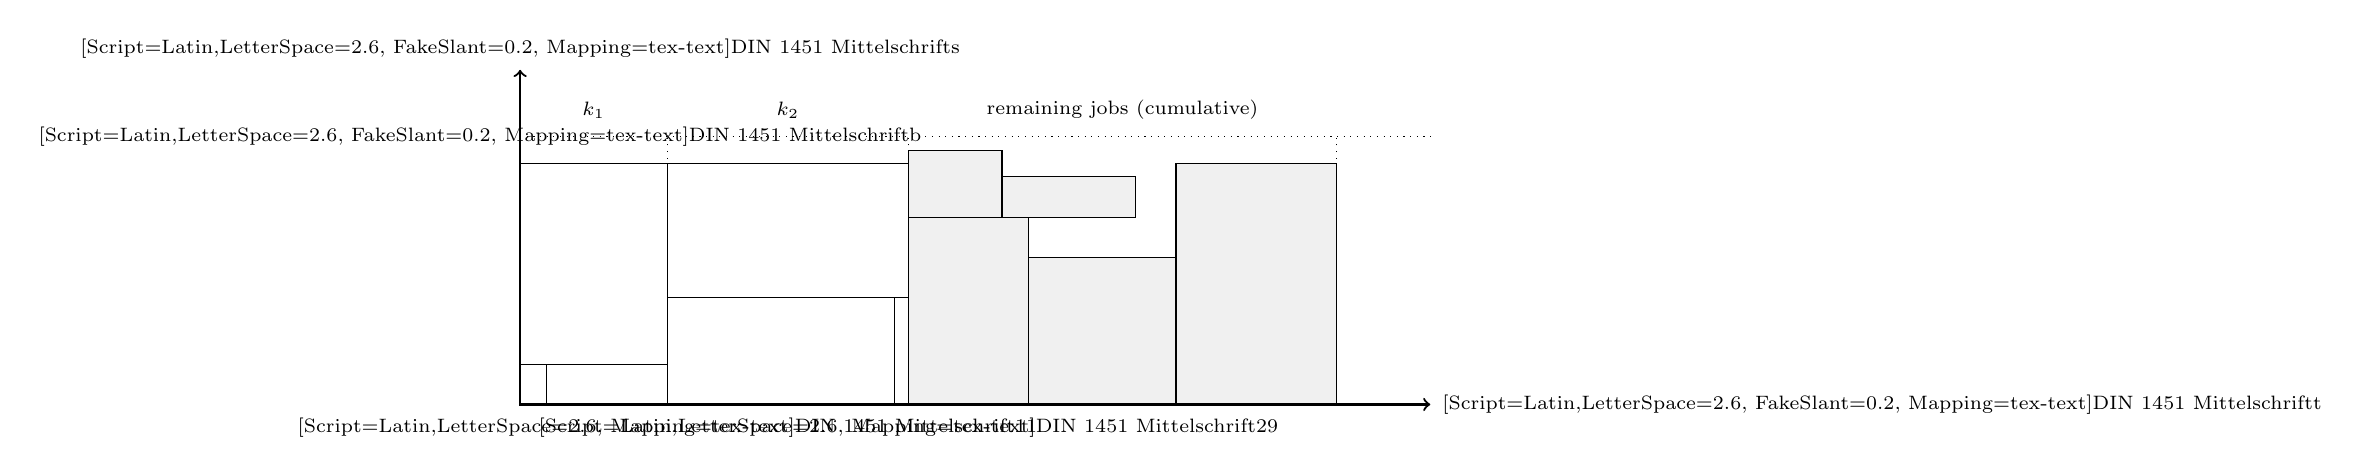
\begin{tikzpicture}[scale=0.17, font=\scriptsize]
            \draw[dotted] (0,20) -- (68,20);
      \node at (-3, 20) {{\sansitalicfont b }};
        \draw (0,0) rectangle (2,3) ;
        \draw (0,3) rectangle (11, 18); 
        \node at (5.5, 22) {$k_1$};
        \node at (11, -1.7) {\sansfont 11};
      \draw[dotted] (11,0) -- (11,20); 
        \draw (11,0) rectangle (28, 8) ;
        \draw (11,8) rectangle (29,18);
        \node at (20, 22) {$k_2$};
        \node at (29, -1.7) {\sansfont 29};
      \draw[dotted] (29,0) -- (29, 20);
        \draw[fill={rgb:black,1;white,16}](29,0) rectangle (38,14) ;
        \draw[fill={rgb:black,1;white,16}] (29,14) rectangle (36,19);
        \draw[fill={rgb:black,1;white,16}] (36,14) rectangle (46,17);
        \draw[fill={rgb:black,1;white,16}] (38,0) rectangle (49,11);
        \draw[fill={rgb:black,1;white,16}] (49,0) rectangle (61, 18);
\draw [<->,thick] (0,25) node (yaxis) [above] {\sansitalicfont s}
        |- (68,0) node (xaxis) [right] {\sansitalicfont t};

        \node at (45, 22) {remaining jobs (cumulative)};
      \draw[dotted] (61,0) -- (61, 20);

    \end{tikzpicture}
 \caption{Constructing the second batch. Remaining jobs are shaded.}\label{fig:decomp_tetris}
\end{figure}

We can use a
MIP model at each node to assign jobs to the respective batch. The remaining
jobs are scheduled after the batch such as to minimize their $\Lmax$, with a relaxation of the
batching requirement, i.e., as if on a cumulative resource as illustrated in
Figure \ref{fig:decomp_tetris}. This yields a lower bond $LB(\Lmax)$ on the
value of $\Lmax$, which can be used to prune the search tree (when $LB(\Lmax)$
exceeds the incumbent $L_\text{max,incmb}$).
\begin{model}[h!]
\begin{alignat}{3}
\text{Min.}\quad & L_{\text{max,cumul}} && \\ 
\text{s. t.}\quad & \label{dc:eq1} \sum_j s_j x_j \leq b \quad && \forall j \in J \\
& P_k \geq p_j x_j \quad && \forall j \in J \\
& \label{dc:eq3} \sum_j x_j \geq 1 \quad && \forall \{j \in J | d_j = \min(d_j)\} \\
& \label{dc:eq4} P_k + \frac{1}{b} \sum_{i} (1-x_i) s_i p_i \leq d_j +
L_{\text{max,incmb}} - 1 - v_k \quad && \forall j \in J, \forall \{i \in J | d_i
\leq d_j\} \\[2ex]
& \label{dc:eq5} \sum_t u_{jt} = 1 \quad && \forall j \in J \\
& \label{dc:eq6} \sum_j \sum_{t' \in T_{jt}} s_j u_{jt'} \leq b \quad && \forall t \in \mathcal{H} \\
& \label{dc:eq7} (v_k + t + p_j) u_{jt} \leq d_j + L_{\text{max,incmb}} - 1 \quad && \forall j \in J, \forall t \in \mathcal{H} \\
& \label{dc:eq8} L_{\text{max,cumul}} \geq (v_k + t + p_j) u_{jt} - d_j \quad && \forall j \in J, \forall t \in \mathcal{H} \\
& \label{dc:eq9} u_{j,t=0} = x_j \quad && \forall j \in J \\
& \label{dc:eq10} u_{it} \leq (1 - x_j) \quad && \forall i,j \in J, \forall t
\in \{1, \dots, p_j - 1\} \\[2ex]
& \label{dc:eq11} b - \sum_{i \in J} s_i x_i \leq (b w_j + 1) s_j \quad && \forall j \in J \\
& \label{dc:eq12} P_k + 2w_j n_t \geq p_j + n_t x_j \quad && \forall j \in J\\
& \label{dc:eq13} P_k - 2(1 - w_j)n_t \leq p_j +n_t x_j - 1 \quad && \forall j
\in J
\end{alignat}
\caption{MIP model in batch-by-batch branch-and-bound}
\label{model:decomp_mip}
\end{model}

\begin{table}[h]
\begin{tabular}{l p{5in}}
$x_j$ & is 1 iff job $j$ is assigned to the batch \\
$u_{jt}$ & is 1 iff job $j$ starts in time slot $t$ \\
$T_{jt}$ & is the set of all time slots occupied by job $j$ if it ended at time
$t$, that is $T_{jt} = \{t - p_j + 1, \dots, t\}$ \\
$v_k$ & is the start time of the batch at the given node in the search tree \\
$L_{\text{max,incmb}}$ & is the incumbent (known best) value of and thus an
upper bound on $\Lmax$ \\
$\mathcal{H}$ & is the set of all indexed time points $\{0, \dots, n_t - 1\}$ \\
$w_j$ & is 1 iff job $j$ is either longer than the batch ($p_j > P_k$) or
already part of the batch ($x_j = 1$). Neither condition must be fulfilled for constraint
\eqref{dc:eq11} to have an effect on job $j$
\end{tabular}
\caption{Notation used in the decomposition model}
\end{table}

Model \ref{model:decomp_mip} implements a time-indexed cumulative constraint on the
non-batched jobs. Constraints \eqref{dc:eq1} through \eqref{dc:eq3} ensure that the
batch stays below capacity, define the duration of the batch $P_k$ and force at
least one of the earliest-due jobs into the batch.

Constraints \eqref{dc:eq4} express the interval relaxation as follows: for any
job $j$, the sum of $P_k$, the processing time of the batch, and the
area-relaxed processing time approximation of all non-batched jobs earlier than
and including $j$, must not exceed the latest finish time of $j$.
Even jobs that are assigned to the batch have to fulfill this requirement.

Constraints \eqref{dc:eq5} and \eqref{dc:eq6} implement the cumulative nature of the
post-batch assignments by ensuring that each job starts only once, and no jobs
overlap on a given resource at any time.

Constraints \eqref{dc:eq7} again limit the possible end dates of a
job, but unlike \eqref{dc:eq4}, they use the time assignments on the cumulative
resource to determine end dates. Constraints \eqref{dc:eq8} define the value of
$L_{\text{max,cumul}}$, the maximum lateness of any job in the non-batched set.

Constraints \eqref{dc:eq9} force batched jobs to start at $t = 0$, while
\eqref{dc:eq10} force \textit{all} jobs to start either at $t = 0$ or after the
last batched job ends.

Constraints \eqref{dc:eq11} enforce a dominance rule: jobs must be assigned to
the batch such that the remaining capacity, $b_r = b - \sum_j s_j x_j$, is less
than the size $s_j$ of the \textit{smallest} job from the set of non-batched
jobs that are \textit{not longer} than the current batch. That is, if there
exists an non-batched job $j$ with $p_j \leq P_k$ and $s_j \leq b_r$, then the
current assignment of jobs is infeasible in the model. The reasoning goes as
follows: given any feasible schedule, assume there is a batch $k_a$ with $b_r$
remaining capacity and a later batch $k_b$ containing a job $j$ such that $s_j
\leq b_r$ and $p_j \leq P_{k_a}$. Then job $j$ can always be moved to batch
$k_a$ without negatively affecting the quality of the solution: if the schedule
was optimal, then moving $j$ will not affect $\Lmax$ at all (otherwise, it was
no optimal schedule); if the schedule was not optimal, then $\Lmax$ will stay
constant (unless $j$ was the longest job in $k_b$ and $\Lmax$ occurred in or in a
batch after $k_b$, in which case $\Lmax$ will be improved).

This rule is implemented by means of a binary variable $w_j$, which, as defined
by constraints \eqref{dc:eq11} and \eqref{dc:eq12}, is 1 iff $p_j > P_k \lor x_j
= 1$. These are the cases in which a job $j$ is \textit{not} to be considered in
\eqref{dc:eq10}, and so $w_j$ is used to scale $s_j$ to a value insignificantly
large in the eyes of the constraint's less-than relation.

After a solution is found, a child node in the search tree has run the subtree
and returned (backtracked), a constraint of the form 
\begin{alignat}{2}
& \sum_j x_j + \sum_i (1-x_i) \leq n_j - 1 \quad && \forall \{j \in J | x_j =
1\}, \forall \{i \in J | x_i = 0 \}
\end{alignat}
is added to the model before the solver is called again, to exclude the last
solution from the set of feasible solutions. 

\subsection{Replacing the MIP model with a CP model}\label{sec:cpdecomp}
In an equivalent approach we use CP to select the batch assignments,
again based on a minimized $\Lmax$ among the non-batched jobs. Model
\ref{model:decomp_cp} uses interval variables $j$ to represent the jobs;
time constraints on the jobs (\texttt{est}, \texttt{lft} etc.) are represented as
functions $\startOf(j)$ and $\endOf(j)$ as introduced in Section
\ref{sec:schedulingcp}.

Constraints \eqref{dcp:eq1} through \eqref{dcp:eq4} bi-directionally define the
relationship between a job's $x_j$ and $\startOf(j)$: $x_j = 1$ is equivalent
with a start time of $t = 0$, and $x_j = 0$ is equivalent with a start time of
$t \geq P_k$. The term $\sum_{i \in J} p_i$ is used as a large constant as it is
greater than any job's start time.

Constraint \eqref{dcp:eq8} is equivalent to constraints \eqref{dc:eq11} through
\eqref{dc:eq13} in Model \ref{model:decomp_mip} above. The cumulative constraint
\eqref{dcp:eq9} ensures that jobs do not overlap. 

\begin{model}[h!]
\begin{alignat}{2}
\mathrm{Min.} \quad & \Lmax \quad && \\
\mathrm{s.t.} \quad 
& \label{dcp:eq1} \startOf(j) \geq (1-x_j) P_k \quad && \forall j \in J \\
& \startOf(j) \leq (1-x_j) \sum_{i \in J} p_i \quad && \forall j \in J \\
& x_j \geq \frac{ \frac{1}{2} - \startOf(j) }{ \sum_{i \in J} p_i } \quad &&
\forall j \in J \\
& \label{dcp:eq4} x_j \leq 1+\frac{ \frac{1}{2} - \startOf(j)}{\sum_{i \in J} p_i } \quad &&
\forall j \in J \\
& P_k \geq \underset{j \in J}{\max}(x_j p_j) \quad && \\
& \endOf(j) = d_j + L_{\text{max,incmb}} - 1 \quad && \forall j \in J \\
& \Lmax \geq \underset{j \in J}{\max}(\endOf(j) - d_j) \quad &&  \\
& \label{dcp:eq8} \mathtt{IfThen}(p_j \leq P_k \land x_j = 0, b - \sum_{j \in J} s_j
x_j \leq s_j) \quad && \forall j \in J \\
& P_k + \frac{1}{b} \sum_i s_i p_i \leq d_j + L_{\text{max,incmb}} - 1 - v_k
\quad && \forall j \in J, \forall \{i \in J | d_i \leq d_j\} \\
& \sum_j x_j \geq 1 \quad && \forall \{ j \in J | d_j = \min(d_j) \} \\
& \label{dcp:eq9} \mathtt{cumul}(J, b) \quad & &  
\end{alignat}
\caption{CP model in batch-by-batch branch-and-bound}
\label{model:decomp_cp}
\end{model}

%%%%%%%%%%%%%%%%%%%%%%%%%%%%%%%%%%%%%%%%%%%%%%%%%%%%%%%%%%
%%%%%%%%%%% MOVE-BASED MIP MODEL %%%%%%%%%%%%%%%%%%%%%%%%%
%%%%%%%%%%%%%%%%%%%%%%%%%%%%%%%%%%%%%%%%%%%%%%%%%%%%%%%%%%

\section{Move-based MIP model}
\label{sec:movebackmip}
This approach is based on the idea of preserving EDD ordering among the batches.
Let an initial schedule be the single-EDD schedule as defined in section
\ref{sec:nopostponing}. We can calculate the lateness
$L_{k,\text{single}}$ of every job in this schedule in linear time.

For the purpose of this discussion, we use the following terminology: in any
batch $k$ holding multiple jobs in an EDD schedule, let \textit{host job} denote
the earliest-due job in the batch (i.e., the job for which $j = k$ as it has
not been moved), and \textit{guest jobs} all other jobs in the batch. If a
batch $k$ only holds one job $j$, then job $j$ is said to be \textit{single}.
 
We now observe the following two things:
 
\begin{proposition}
Consider a schedule in which batches are ordered by EDD. Then moving job $j$
from batch $k_\beta$ into an earlier batch $k_\alpha$ will preserve EDD ordering
if $j$ is single in $k_\beta$ and if $k_\alpha$ is not empty.
\end{proposition}
\begin{proof}
Moving $j$ into $k_\alpha$ will leave $D_\alpha$ unaffected, since $k_\alpha$ is
not empty, i.e. there is a host job in $k_\alpha$. Since the original schedule
was EDD-ordered, the host in $k_\alpha$ is due earlier than $j$. Note that if
$k_\alpha$ is empty, the move will potentially disrupt EDD ordering, and is thus
prohibited.
 
Batch $k_\beta$ will be reduced to zero processing time, but batches after
$k_\beta$ will still be due after $k_{\beta - 1}$, so EDD ordering is preserved.
\end{proof}
 
\begin{proposition}
Starting from a single-EDD schedule, moving single jobs into earlier
non-empty batches allows us to generate all possible EDD schedules, with the exception
of those EDD schedules in which two hosts of the same due date are sorted in
order of decreasing processing time.
\end{proposition}
\begin{proof}
The order in which moves are performed is arbitrary; moves are independent of
each other (capacity requirements notwithstanding). Therefore, any job can be
moved into any earlier bucket (i.e. set of batches of equal due date). Within
buckets, jobs are free to move with the only condition that host jobs be sorted
by non-decreasing processing time, as given by the initial single-EDD schedule.
Under this condition, then, all possible EDD schedules can be generated by
moving single jobs into earlier batches. \end{proof}

\begin{figure}
  \centering
    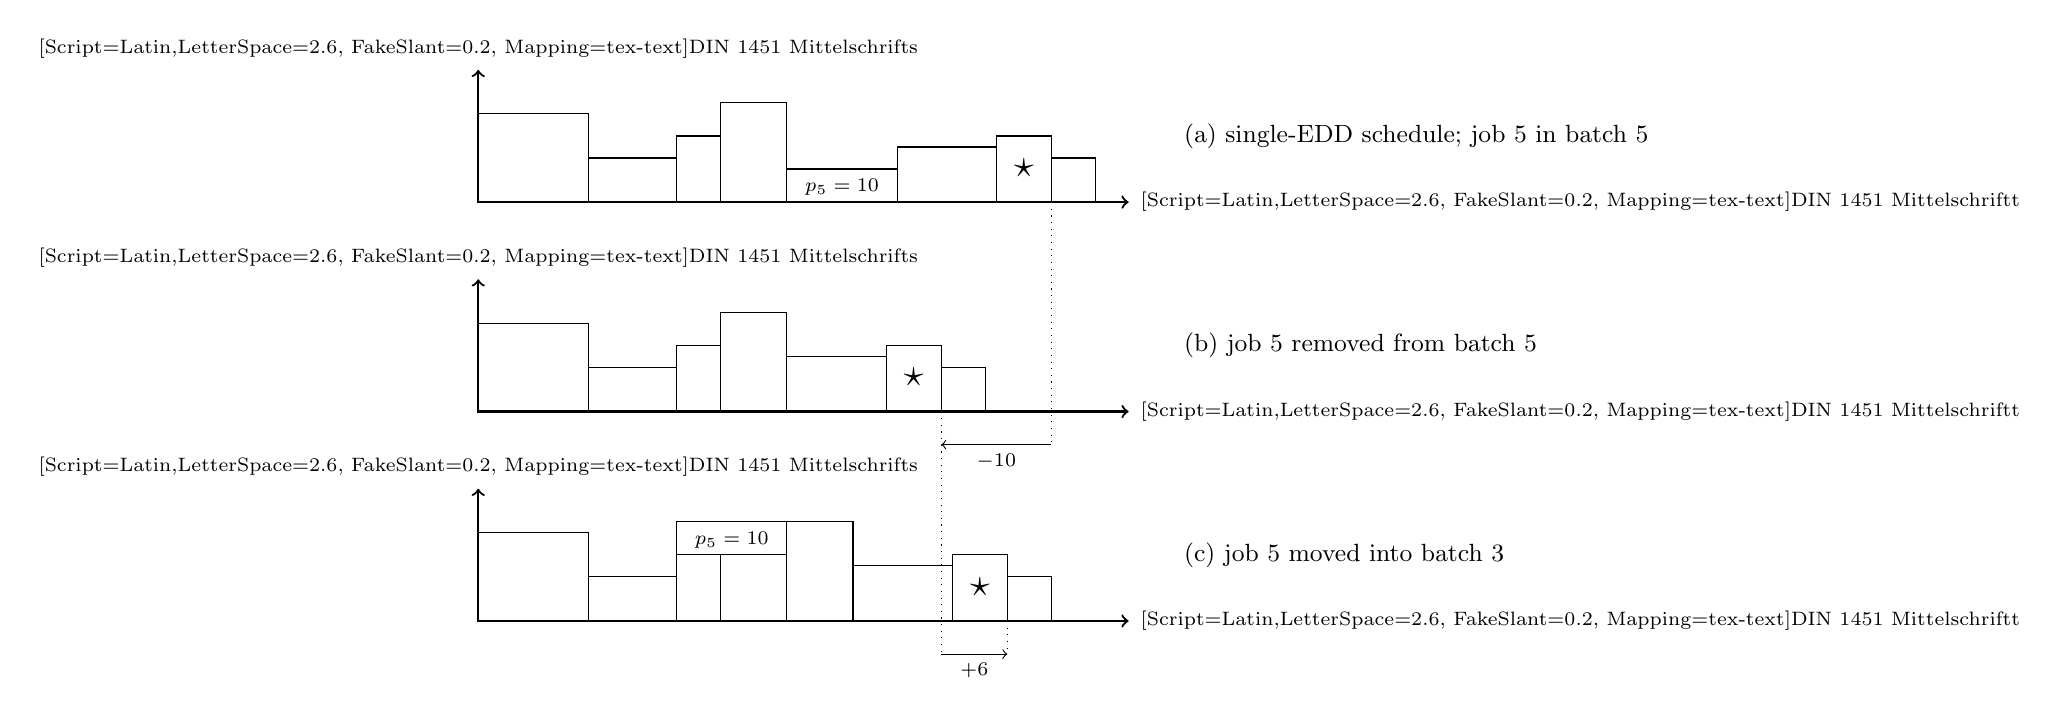
\begin{tikzpicture}[scale=0.14, font=\scriptsize]
    \draw [<->,thick] (0,12) node (yaxis) [above] {\sansitalicfont s}
        |- (59,0) node (xaxis) [right] {\sansitalicfont t};
        \draw (0,0) rectangle (10,8) ;
        \draw (10,0) rectangle (18,4) ;
        \draw (18,0) rectangle (22,6) ;
        \draw (22,0) rectangle (28,9) ;
        \draw (28,0) rectangle (38,3) node[fn,yshift=-3pt] {$p_5 = 10$};
        \draw (38,0) rectangle (47,5) ;
        \draw (47,0) rectangle (52,6) node[fn,yshift=-3pt] {\Large$\star$};
        \draw (52,0) rectangle (56,4) ;
     
      \draw[dotted] (52,0) -- (52,-22); 
    \node[anchor=west] at (63,6) {\small (a) single-EDD schedule; job 5 in batch
    5};

  \begin{scope}[shift={(0,-19)}]
     \draw [<->,thick] (0,12) node (yaxis) [above] {\sansitalicfont s}
        |- (59,0) node (xaxis) [right] {\sansitalicfont t};
        \draw (0,0) rectangle (10,8) ;
        \draw (10,0) rectangle (18,4) ;
        \draw (18,0) rectangle (22,6) ;
        \draw (22,0) rectangle (28,9) ;
        \draw (28,0) rectangle (37,5) ;
        \draw (37,0) rectangle (42,6) node[fn,yshift=-3pt] {\Large$\star$};
        \draw (42,0) rectangle (46,4) ;

    \node[anchor=west] at (63,6) {\small (b) job 5 removed from batch 5};
        \draw[dotted] (42,0) -- (42, -22);
        \draw[<-] (42,-3) -- (52,-3) node[fn, yshift=-8pt] {$-10$};
  \end{scope}

  \begin{scope}[shift={(0,-38)}]
     \draw [<->,thick] (0,12) node (yaxis) [above] {\sansitalicfont s}
        |- (59,0) node (xaxis) [right] {\sansitalicfont t};
        \draw (0,0) rectangle (10,8) ;
        \draw (10,0) rectangle (18,4) ;
        \draw (18,0) rectangle (22,6) ;
        \draw (18,6) rectangle (28,9) node[fn,yshift=-3pt] {$p_5 = 10$} ;
        \draw (28,0) rectangle (34,9) ;
        \draw (34,0) rectangle (43,5) ;
        \draw (43,0) rectangle (48,6) node[fn,yshift=-3pt] {\Large$\star$};
        \draw (48,0) rectangle (52,4) ;

    \node[anchor=west] at (63,6) {\small (c) job 5 moved into batch 3};
        \draw[dotted] (48,0) -- (48, -3);
        \draw[->] (42,-3) -- (48,-3) node[fn, yshift=-8pt] {$+6$};
  \end{scope}

        
    \end{tikzpicture}
 \caption{Moving a job in the move-based MIP. In this example, job 5 (marked
``$p_5 = 10$'') is moved
 into batch 3, which changes the lateness of job 7 (marked
 \Large$\star$\normalsize) from $L_{7,\text{single}}$ to $L_{7,\text{single}} -
 10 + 6 = L_{7,\text{single}} - 4$.}\label{fig:movebasedmip}
\end{figure}


Consider now a single-EDD schedule (Figure \ref{fig:movebasedmip}a). Moving $j$ from its single-EDD batch $k_j$ into an earlier
batch $k_\alpha$ has the following effect:
\begin{alist}
\item{the lateness of all batches after $k_j$ is reduced by $p_j$ (Figure
\ref{fig:movebasedmip}b),}
\item{the lateness of all batches after $k_\alpha$, including those after $k_j$,
is increased by $\max(0,p_j - P_\alpha)$, where $P_\alpha$ is the processing
time of batch $\alpha$ before $j$ is moved into it (Figure
\ref{fig:movebasedmip}c).}
\end{alist}
Since, in any batch $k$, only the host job's lateness (with index $j = k$) is
relevant to $\Lmax$, we can understand the lateness of batch $k$ as the
single-EDD lateness of job $k = L_{k,\text{single}}$, modified by summed effect
all moves of other jobs into and out of earlier batches have on $k$, as listed
above.
 
The following expression defines the lateness of a batch $k$ based on this
calculation:
 
\begin{alignat}{2} & L_k = L_{k,\text{single}} - \sum_{h=0}^{k} P_h - p_h(2 -
x_{hh}) \quad && \forall k \in K^\star \end{alignat}
 
where $x_{jk}$ is 1 iff job $j$ is assigned to batch $k$ in the solution
schedule. The sum term represents the effects that all moves have on previous
batches up to and including $k$: $x_{hh} = 1$ iff job $h$ is not moved from
its single-EDD batch $h$, and so the sum term evaluates to $P_h - p_h$ for a
batch in which the host was not moved. If $h$ has guests, then $P_h - p_h$ is
positive if any of the guests is longer than $j_h$ (i.e. $P_h > p_h$); if not,
or if $h$ has no guests at all, it will be zero. Effectively thus, for batch
$h$, the time $\max(0, P_h-p_h)$ is added to $L_k$. If, however, job $h$ was
moved out of its batch, then the batch will have a processing time of $P_h =
p_h$ (the fixed lower bound for $P_h$). In this case, effectively, for batch
$h$, the time $p_h$ is subtracted from $L_k$. The net sum of these additions
and subtractions to and from $L_{k,\text{single}}$ adjusts the lateness of
batch $k$ to its correct number given the values of $x_{jk}$. 

Note also that we only need to calculate the lateness for $k \in K^\star$, the set
of batches that are the last in their respective buckets; in other words, those
with the longest processing time in their respective bucket. This is true
because empty batches in a bucket will be reduced to length $P = 0$ by the
minimization objective.

The full set of constraints is listed in Model \ref{mod:movebackmip}, and the
following section explains every constraint in detail.
\begin{model}
\begin{alignat}{2}
\text{Min.}\quad & \Lmax && \\
\text{s.t.}\quad & \label{mbm:eq7}\sum_{k} x_{jk} = 1 \quad && \forall j \in J \\
& \label{mbm:eq6}\sum_{j} s_j x_{jk} \leq b \quad && \forall k \in K \\
&\label{mbm:eq3} P_k \geq p_j x_{jk} \quad && \forall \{j \in J, k \in K | j \geq k\} \\
&\label{mbm:eq5} x_{jk} \leq x_{kk} \quad && \forall \{j \in J, k \in K | j > k\} \\
&\label{mbm:eq4} \Lmax \geq L_{k,\text{single}} - \sum_{h=0}^{k} P_h - p_h(2 -
x_{hh}) \quad && \forall k \in K^\star \\
\label{mbm:eq1} & x_{jk} = 0 \quad && \forall \{j \in J, k \in K | j > k\} \\
&\label{mbm:eq2} x_{jj} = 1 \quad && \forall \{j \in J | j \geq f_L\} \\[2ex]
(*)\quad & \label{mbm:eq8}\begin{gathered} 2(  4 - x_{k_1,k_1} - x_{k_2,k_2} \hfill \\+ \sum_{\substack{{j}\\{j \neq j_1}\\{j \neq
j_2}}} - x_{j_1,k_1} - x_{j_1,k_2} -
x_{j_2,k_1} - x_{j_2,k_2} ) \geq x_{j_1,k_2} + x_{j_2,k_1} \end{gathered}
\quad && \begin{gathered} \forall\{ j_1, j_2 \in J, \\ k_1, k_2 \in K \\|\; k_1 < k_2 <
j_1 < j_2 \land \\ [p_i \leq k_h \land b - s_h \geq s_i\\ \forall i \in
\{j_1,j_2\}, \\ \forall h
\in \{k_1,k_2\}] \} \end{gathered} \\[2ex]
(*)\quad & \label{mbm:eq9}1-x_{j_1,j_1} \geq x_{j_2,k} \quad && \begin{gathered} \forall \{k \in K,
j_1 \in J, j_2 \in J \\|\; k < j_1 < j_2 \\ \land s_{j_1} \leq s_{j_2} \\
\land s_{j_2} + s_k \leq b \\ p_{j_1} \leq p_k 
\land p_{j_1} \geq p_{j_2} \} \\
\end{gathered} \\[2ex]
(*)\quad &  \label{mbm:eq11}2 - x_{jj} - x_{kk} \geq \left(1.0 + b - s_j -
\sum_{\substack{{i = k}\\{i \neq j}}}^{n_j} s_i
x_{ik}\right) / b \quad && \begin{gathered} \forall \{k \in K, j \in J \\| j > k 
\land p_k \geq p_j \\ \land s_k + s_j \leq b\}\end{gathered}
\end{alignat}
\caption{Move-based MIP model. Constraints marked $(*)$ are lazy constraints
(see Section \ref{sec:lazyconstraints} for details).}
\label{mod:movebackmip}
\end{model}
Constraints \eqref{mbm:eq6} and \eqref{mbm:eq7} are capacity constraints and
uniqueness constraints: batches have to remain within capacity $b$, and every
job can only occupy one batch.

Constraints \eqref{mbm:eq3} define the value of $P_k$ for every batch $k$ as the
longest $p$ of all jobs in $k$. This is required in the definition of batch
lateness as described above and also in \eqref{mbm:eq4}, which follows the
explanation above.

Constraints \eqref{mbm:eq5} ensure that no job is moved into a host-less batch,
i.e. in order to move job $j$ into batch $k$ ($x_{jk} = 1$), job $k$ must still
be in batch $k$ ($x_{kk} = 1$).

Constraints \eqref{mbm:eq1} implement the requirement that jobs are only moved
into earlier batches.

Constraints \eqref{mbm:eq2} apply to jobs with index greater than $f_L$, which
is the index of the job with the largest value for $L_{k,\text{single}}$. All
jobs after batch $f_L$ can be ignored in the question, based on the proof given in
Appendix \ref{sec:movebackproof}. This constraint fixes those jobs to their
single-EDD batches, effectively removing them from the model. This set of
constraints is rarely active but can greatly decrease the size of the model in
some instances.

Constraints \eqref{mbm:eq8} through \eqref{mbm:eq11} are dominance rules
implemented as lazy constraints as defined in subsection
\ref{sec:lazyconstraints}, and are presented in greater length in the following
subsections.

\subsection{Symmetry-breaking rule}
Constraints \eqref{mbm:eq8} implement the following concept: if two jobs $j_1$
and $j_2$ are assigned as guests to batches $k_1$ and $k_2$, and no other jobs
(save for the hosts) are assigned to $k_1$ and $k_2$, then $j_1$ is always
assigned to $k_1$ and $j_2$ to $k_2$. These constraints only hold for pairs of
jobs where both $p_{j_1}$ and $p_{j_2}$ are less than both $p_{k_1}$ and
$p_{k_2}$ (both batches are longer than the jobs) and all possible assignments
are feasible capacity-wise.

Large problem instances generate thousands of such constraints, and only very
few of them will ever hold in the model. Nevertheless, they can noticeably
improve solving time in some cases; declaring them as ``lazy'' helps keep
the model small.

\subsection{Dominance rule on ``safe'' moves}
\label{sec:dominance-safe}
For the following sections, note that a \textit{safe} move is defined as one
where the guest job is shorter than the host job ($p_\text{guest} \leq
p_\text{host}$), i.e. a move that will under no circumstances increase the
processing time of the host job.

This applies to pairs of jobs $j_1 < j_2$ that are, potentially, competing
to be guests in batch $k$. If both $j_1$ and $j_2$ are shorter (in terms of $p$)
than $k$, we can safely enforce that in some cases, $j_1$ gets priority over
$j_2$, namely if both $p_{j_1} \geq p_{j_2}$ and $s_{j_1} \leq s_{j_2}$ hold. In
this case, we can state that $j_2$ cannot be moved into $k$ unless $j_1$ has
been moved somewhere also (into $k$ or some other host batch).

Two facts allow for this set of rules:
\begin{proposition}If a job $j_h$ can either be safely moved into an earlier batch,
\textrm{or} act as a host for later jobs $J_g = \{j_{g_1}, j_{g_2}, \dots\}$,
moving $j_h$ is always preferable. \label{prop:moveisbetter}

\begin{proof}
Let $k_{\Lmax}$ be the batch hosting the job with maximum lateness in the final
solution. If $j_h$ is due after $k_{\Lmax}$, moving it will have no impact on
$\Lmax$ (see Appendix \ref{sec:movebackproof}). If $j_h$ is due before
$k_{\Lmax}$, but the earliest-due of $J_g$ is due after $k_{\Lmax}$, then moving
$J_g$ into $j_h$ will have no impact or a worsening impact on $\Lmax$. If both
$j_h$ and $J_g$ are due before $k_{\Lmax}$, then moving $J_g$ will, at best,
improve $\Lmax$ by $p_{j_h}$ (if $\underset{p}{\max}(J_g) \geq p_{j_h}$). In
this case, however, moving $j_h$ back safely will, under any circumstances,
reduce $\Lmax$ by $p_{j_h}$. The first job in $J_g$ can host all later jobs in
$J_g$ (and possibly more, since vertical capacity was freed). The total
reduction in $\Lmax$ in this case is improved.
\end{proof}
\end{proposition}

\begin{proposition} If a job $j_1$ with $d_{j_1} \leq d_{j_2}$ is both longer
and thinner than $j_2$ ($p_{j_1} \geq p_{j_2}, s_{j_1} \leq s_{j_2}$), assigning
it as a guest to $k$ will produce a lower $\Lmax$ than assigning $j_2$ to $k$.

\begin{proof}
Because of due date and size requirements, $j_1$ is a potential host for $j_2$,
Proposition \ref{prop:moveisbetter} applies. 

Generally, a longer guest job will result in a greater reduction in $\Lmax$, and
is thus preferable. Since $j_1$ is thinner than $j_2$, the dominance rule will
not preclude (via capacity constraints) other guest jobs from being assigned to
$k$ as a consequence of prioritizing $j_1$ over $j_2$.
\end{proof}
\end{proposition}

\subsection{Dominance rule on required safe moves}
This constraint can be expressed logically as: if $j$ can be safely moved into $k$
without violating the capacity constraint, then $j$ must be moved somewhere, or
$k$ must be empty (or both). In other words, in the context of Proposition
\ref{prop:moveisbetter}, a schedule is unacceptable if job $j$ is left in its
single-EDD batch although there is room for it in an earlier batch.

The left side of the above \textit{if-then} statement is written as $(b + 1 -
s_j - \sum_{\substack{{i = k}\\{i \neq j}}}^{n_j} s_i x_{ik}) / b$, which
evaluates to 1.0 or greater iff $s_k$ plus the sizes of guest jobs in $k$ sum to
less than $b - s_j$.




\chapter[Empirical comparison of models]{Empirical comparison\\ of models}
\section{Experimental setup}
The models were tested on a set of job lists. Malapert's paper uses benchmark
job lists by \citet{Daste1, Daste2}, with a capacity of $b = 10$ and values for
$p_j$, $s_j$ and $d_j$ distributed as follows:
\begin{align}
p_j &= U[1, 99] \\
s_j &= U[1, 10] \\
d_j &= U[0, 0.1] \cdot \tilde{C}_\text{max} + U[1, 3] \cdot p_j
\end{align}
where $U[a, b]$ is a uniform distribution between $a$ and $b$, and $\tilde{C}_\text{max} = \left( \sum_{j=1}^{n_j} s_j \cdot \sum_{j=1}^{n_j}
p_j \right) /\\ (b \cdot n)$ is an approximation of the time required to process
all jobs.

Ten different sample job sets are
used per unique value of $n_j \in \{10, 11, \dots, 18, 19, 20, 25,\\ 30, 35, 40, 45, 50\}$. The times shown in figure \ref{fig:comp_times}
are averaged over those ten instances for each $n_j$.

The models were run using Cplex 12.2 \citep{cplex} on an Intel i7 Q740 CPU (1.73 GHz) in single-thread mode, with 8 GB RAM.
Solving was aborted after a time of 3600 seconds (1 hour).

\section{Results}
\label{sec:results}
The CP branch-and-bound model (Model \ref{model:decomp_cp}) times out on most instances and is not shown here.
The pure CP model (Model \ref{model:cpmodel}) times out on one 12-job instance and gets progressively worse
with more jobs; similar to Malapert's original MIP model.
\begin{figure}
\centering

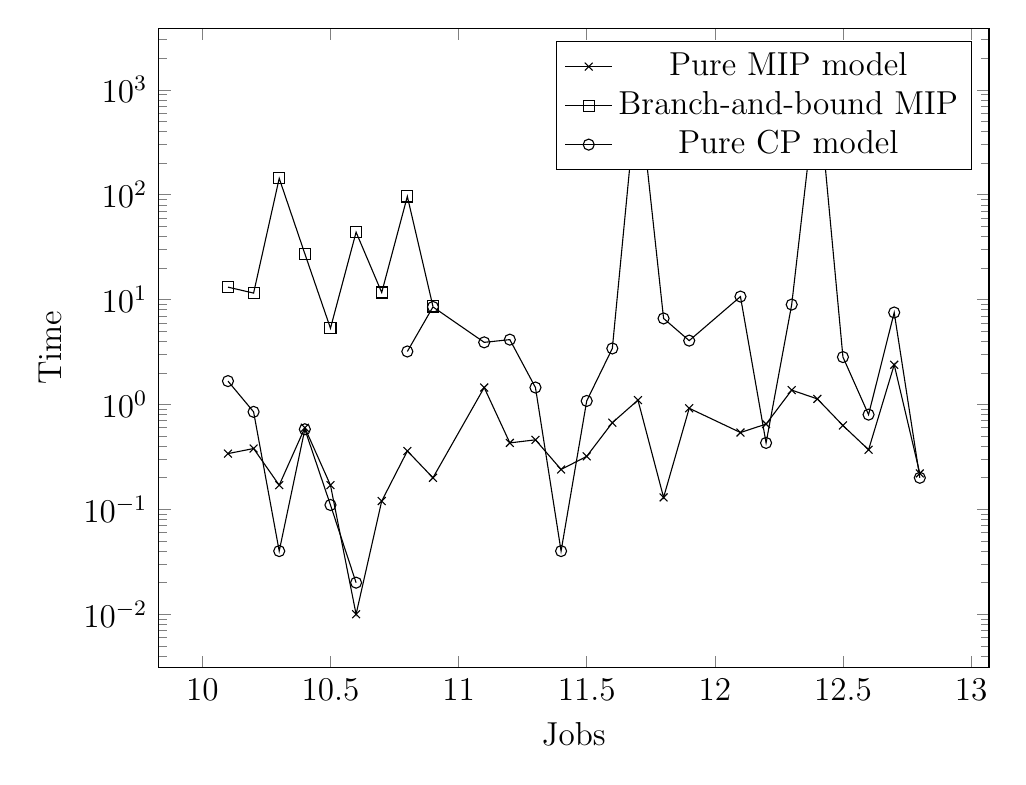
\begin{tikzpicture}
  \begin{semilogyaxis}[xlabel=Jobs, ylabel=Time, width=\textwidth,
  height=0.8\textwidth]
  \addplot[color=black, mark=x ] coordinates { % MIP model times
(10.1, 0.34)
(10.2, 0.38)
(10.3, 0.17)
(10.4, 0.6)
(10.5, 0.17)
(10.6, 0.01)
(10.7, 0.12)
(10.8, 0.36)
(10.9, 0.2)
(11.1, 1.45)
(11.2, 0.43)
(11.3, 0.46)
(11.4, 0.24)
(11.5, 0.32)
(11.6, 0.67)
(11.7, 1.1)
(11.8, 0.13)
(11.9, 0.92)
(12.1, 0.54)
(12.2, 0.65)
(12.3, 1.37)
(12.4, 1.13)
(12.5, 0.63)
(12.6, 0.37)
(12.7, 2.39)
(12.8, 0.22)
  };
  \addlegendentry{Pure MIP model}
  \addplot[color=black, mark=square] coordinates {
(10.1, 13.14)
(10.2, 11.53)
(10.3, 143.11)
(10.4, 27.34)
(10.5, 5.33)
(10.6, 43.9)
(10.7, 11.68)
(10.8, 96.27)
(10.9, 8.6)
  };
  \addlegendentry{Branch-and-bound MIP}
  \addplot[color=black, mark=o] coordinates {
(10.1, 1.67)
(10.2, 0.85)
(10.3, 0.04)
(10.4, 0.58)
(10.5, 0.11)
(10.6, 0.02)

(10.8, 3.2)
(10.9, 8.51)
(11.1, 3.91)
(11.2, 4.15)
(11.3, 1.45)
(11.4, 0.04)
(11.5, 1.08)
(11.6, 3.42)
(11.7, 1200)
(11.8, 6.61)
(11.9, 4.06)
(12.1, 10.68)
(12.2, 0.43)
(12.3, 8.96)
(12.4, 1200)
(12.5, 2.83)
(12.6, 0.8)
(12.7, 7.53)
(12.8, 0.2)
};
  \addlegendentry{Pure CP model}
  \end{semilogyaxis}
\end{tikzpicture}

\caption{Comparison of CPU time used by different models.}
\label{fig:comp_times}
\end{figure}

 The new, move-based MIP model (Model
\ref{mod:movebackmip}) trumps all other
models' performance by at least one order of magnitude.

Unfortunately we have no such performance profile for Malapert's
\texttt{sequenceEDD} global constraint. We do, however, have a reference in
Figure \ref{fig:malapertresultcomp}, which shows the percentage of solved
problem instances in a given time. The figure is based on $n_j \in \{10, 20,
50\}$, with 40 instances each (120 instances total).
\begin{figure}
  \centering
    \noindent\begin{tikzpicture}
    \node[anchor=south west, inner sep=0] at (-3pt,-1pt)
    {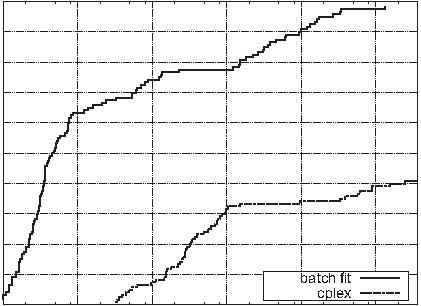
\includegraphics[width=0.9\textwidth]{figures/malapertfinal.pdf}};

  \begin{semilogxaxis}[width=0.99\textwidth, 
  height=0.749\textwidth,legend pos=south east, xmin=0.01, xmax=3600, ymin=0,
  ymax=1.0, xtick={0.01, 0.1, 1, 10, 100, 1000, 3600}, ytick={0, 0.1, 0.2, 0.3,
  0.4, 0.5, 0.6, 0.7, 0.8, 0.9, 1.0}, x tick label style={
        /pgf/number format/.cd,
            fixed,
            fixed zerofill,
            precision=2,
        /tikz/.cd
    }, log ticks with fixed point, 
    every axis legend/.append style={xshift=8pt, yshift=-5pt}]
  \addplot[color=black, mark=none] coordinates {
(0.01, 0.175)
(0.02, 0.291666666666667)
(0.03, 0.325)
(0.04, 0.333333333333333)
(0.05, 0.35)
(0.06, 0.358333333333333)
(0.07, 0.375)
(0.08, 0.4)
(0.09, 0.408333333333333)
(0.1, 0.408333333333333)
(0.2, 0.475)
(0.3, 0.5)
(0.4, 0.533333333333333)
(0.5, 0.558333333333333)
(0.6, 0.566666666666667)
(0.7, 0.566666666666667)
(0.8, 0.566666666666667)
(0.9, 0.575)
(1, 0.575)
(1.2, 0.591666666666667)
(1.5, 0.616666666666667)
(1.6, 0.641666666666667)
(1.8, 0.65)
(2, 0.65)
(2.5, 0.65)
(3, 0.65)
(4, 0.658333333333333)
(5, 0.658333333333333)
(6, 0.683333333333333)
(7, 0.725)
(8, 0.75)
(9, 0.758333333333333)
(10, 0.783333333333333)
(12, 0.816666666666667)
(14, 0.825)
(16, 0.825)
(18, 0.833333333333333)
(20, 0.833333333333333)
(25, 0.85)
(30, 0.866666666666667)
(35, 0.875)
(40, 0.875)
(45, 0.875)
(50, 0.875)
(60, 0.925)
(70, 0.933333333333333)
(80, 0.933333333333333)
(90, 0.933333333333333)
(100, 0.941666666666667)
(120, 0.941666666666667)
(140, 0.95)
(160, 0.95)
(180, 0.95)
(200, 0.95)
(220, 0.95)
(240, 0.95)
(260, 0.95)
(280, 0.95)
(300, 0.95)
(340, 0.95)
(380, 0.95)
(420, 0.95)
(480, 0.95)
(540, 0.958333333333333)
(600, 0.958333333333333)
(650, 0.958333333333333)
(700, 0.958333333333333)
(800, 0.958333333333333)
(900, 0.966666666666667)
(1000, 0.975)
(1200, 0.975)
(1400, 0.975)
(1600, 0.975)
(1800, 0.975)
(2000, 0.975)
(2500, 0.975)
(3000, 0.975)
(3600, 0.975)
};
\addlegendentry{Move-based MIP model}

\addplot[color=black, mark=none, thick] coordinates {(0,0) (1, 0)};
\addlegendentry{\texttt{sequenceEDD} with batch fit heuristic}

\addplot[color=black, mark=none, dashed] coordinates {(0,0) (1,0)};
\addlegendentry{Original MIP}

  \end{semilogxaxis}
\end{tikzpicture}
   \vspace{0.73em}
\caption{Percentage of problem instances solved in a given
time}\label{fig:malapertresultcomp}
\end{figure}


Note that fully tabulated results are given in Appendix \ref{appendix:results}.

\section{Discussion}\label{sec:discussion}
The move-based MIP model uses the fewest variables (columns) and
constraints (rows) and performs the best. The use of lazy constraints for
larger $n_j$ is advantageous in the large majority of problem instances and thus
warranted. 

The improvements made to the original MIP in Model \ref{model:improvedmip} show
a substantial benefit, mostly owed to constraint \eqref{eq:mipnopp} which
excludes a large number of potential batch assignments.

The batch-by-batch decomposition using MIP to assemble batches, while an
improvement over Malapert's MIP model, is not satisfactory; the relaxations are
too lax for the decomposition to compensate for the overhead of a naive
branch-and-bound search, since we can only exclude one failed solution at a
time.

\subsection{Comparison with Malapert's sequenceEDD global constraint}
Using all four filtering rules in conjunction with a \textit{batch fit} search
heuristic allowed Malapert to solve 38 out of 40 problem instances with $n_j =
50$ in less than an hour on a cluster of Linux machines, each node of which
using 48 GB of RAM and two quad core 2.4 GHz processors (that is, using
considerably more powerful hardware than was used for this thesis). 

The move-based MIP model is able to achieve a comparable performance (39 of 40
instances solved within an hour). While it is, on average, slower on problems
with low $n_j$ (compare Figure \ref{fig:malapertresultcomp}), it is able to
prove optimality quicker on most instances that take longer than 10 seconds to
solve---ostensibly the more critical metric.

\section{Further performance tests}
A better understanding of the relationships between model performance and
problem instance characteristics can help in the development of faster models.
This is especially true with regard to redundant and/or lazy constraints that
are used only to achieve a tighter formulation at the price of a larger model:
using such constraints is often warranted only for particularly challenging
problem instances. The following paragraphs outline some such considerations.

\subsection{Correlation between disjunctivity and solving time}
\label{sec:disjunctivity}
The mean number of jobs per batch ($n_j/n_k$) in the optimal solution is
strongly correlated with the time needed to solve to
optimality. This is unsurprising given that a problem with a great number of large
jobs (i.e. large $s_j$) will be of relatively low
difficulty in terms of bin packing. This is illustrated by Figure
\ref{fig:jpbtimecor_a}.
\begin{figure}
\centering
\begin{subfigure}[b]{0.4\textwidth}
  \centering
    \noindent\begin{tikzpicture}
  \begin{semilogyaxis}[ 
  font=\small, width=0.99\textwidth]
  \addplot[color=black, only marks] coordinates {
(1.875, 1.84)
(1.875, 2.45)
(2, 3.3)
(2, 2.14286)
(2.30769, 15.56)
(1.5, 0.44)
(2.14286, 10.33)
(1.76471, 1.99)
(1.6666, 1.78)
(1.5, 0.51)
(1.666667, 1.15)
(1.875, 2.34)
(1.66667, 1.9)
(2, 2.73)
(2.14286, 11.56)
(1.66667, 2.09)
(1.6667, 0.89)
(1.57895, 0.75)
(1.42857, 0.09)
(2, 2.36)
(1.66667, 1.76)
(2, 2.35)
(1.76471, 0.67)
(1.76471, 1.11)
(2.14286, 3.83)
(2, 3.59)
(2.30769, 7.32)
(2, 1.71)
(2, 6.82)
(1.5, 0.41)
(1.76471, 1.29)
(1.875, 2.62)
(2, 2.15)
(1.76471, 2.44)
(2, 4.86)
(2, 1.53)
(2.14286, 4.23)
(1.57895, 1.43)
(1.875, 1.2)
};
  \end{semilogyaxis}
\end{tikzpicture}
\caption{$n_j/n_k$}
\label{fig:jpbtimecor_a}
\end{subfigure}
  \begin{subfigure}[b]{0.4\textwidth}
  \centering
    \noindent\begin{tikzpicture}
  \begin{semilogyaxis}[font=\small, width=0.99\textwidth]
  \addplot[color=black, only marks] coordinates {
(0.407777777778, 1.84)
(0.446666666667, 2.45)
(0.347777777778, 3.3)
(0.337777777778, 2.14286)
(0.296666666667, 15.56)
(0.583333333333, 0.44)
(0.272222222222, 10.33)
(0.398888888889, 1.99)
(0.502222222222, 1.78)
(0.584444444444, 0.51)
(0.536666666667, 1.15)
(0.427777777778, 2.34)
(0.538888888889, 1.9)
(0.346666666667, 2.73)
(0.311111111111, 11.56)
(0.512222222222, 2.09)
(0.524444444444, 0.89)
(0.558888888889, 0.75)
(0.648888888889, 0.09)
(0.397777777778, 2.36)
(0.478888888889, 1.76)
(0.364444444444, 2.35)
(0.487777777778, 0.67)
(0.471111111111, 1.11)
(0.297777777778, 3.83)
(0.354444444444, 3.59)
(0.251111111111, 7.32)
(0.362222222222, 1.71)
(0.294444444444, 6.82)
(0.671111111111, 0.41)
(0.516666666667, 1.29)
(0.428888888889, 2.62)
(0.395555555556, 2.15)
(0.392222222222, 2.44)
(0.312222222222, 4.86)
(0.37, 1.53)
(0.297777777778, 4.23)
(0.525555555556, 1.43)
(0.348888888889, 1.2)
};
  \end{semilogyaxis}
\end{tikzpicture}
\caption{Disjunction ratio}
\label{fig:jpbtimecorb}
  \end{subfigure}
  \caption{Correlation between time to prove optimality in
  seconds (ordinates) and measures of disjunctivity (abscissae), based
  on 40 instances with $n_j=30$. Subfigure (a) shows the average number of jobs
  per batch in the optimal solution. Subfigure (b) shows the \textit{disjunction
  ratio} as defined in Section \ref{sec:disjunctivity}.}
  \label{fig:jpbtimecor}
  
\end{figure}

An excellent predictor of this correlation appears to be what \citet{baptistelepape} call \textit{disjunction ratio}: the ratio between the
number of job pairs which cannot run in parallel (as $s_{j_1} + s_{j_2} > b$) and
the total number of job pairs $n_j^2$.\footnote{The term originates from the
dichotomy between \textit{disjunctive resources} which can only process one job
at a time, and \textit{(highly) cumulative resources} which can process many
jobs in parallel.} The relationship is shown in Figure
\ref{fig:jpbtimecorb}.

As a corollary to the above, the solving time is greatly dependent on the
capacity of the machine. Larger capacities, relative to the average job size
$\bar{s}_j$, will cause longer solving times as the disjunction ratio decreases.

\subsection{Uniform distribution of due dates}
The due dates in the test instances used by Malapert and in the previous tests
were generated by a fairly complex formula designed such that jobs are likely to
fall into \textit{buckets}, i.e. larger sets of jobs with equal due dates.

Malapert's \texttt{sequenceEDD} global constraint exploits the notion of buckets
extensively, and would likely perform worse on instances that exhibit no
bucketing at all (though we could not test this for lack of a working
implementation).

Our move-based model uses only the latest-due batch in every bucket to define
the value of $\Lmax$. As a result, the size of the model is directly dependent
on the number of buckets. We were, however, unable to find evidence of such a
relationship: Figure \ref{fig:uniformddtimecor} shows the performance of the
move-based MIP on non-bucketed ($d_j = U[1, 99]$) instances compared to bucketed
instances. \begin{figure}
\centering

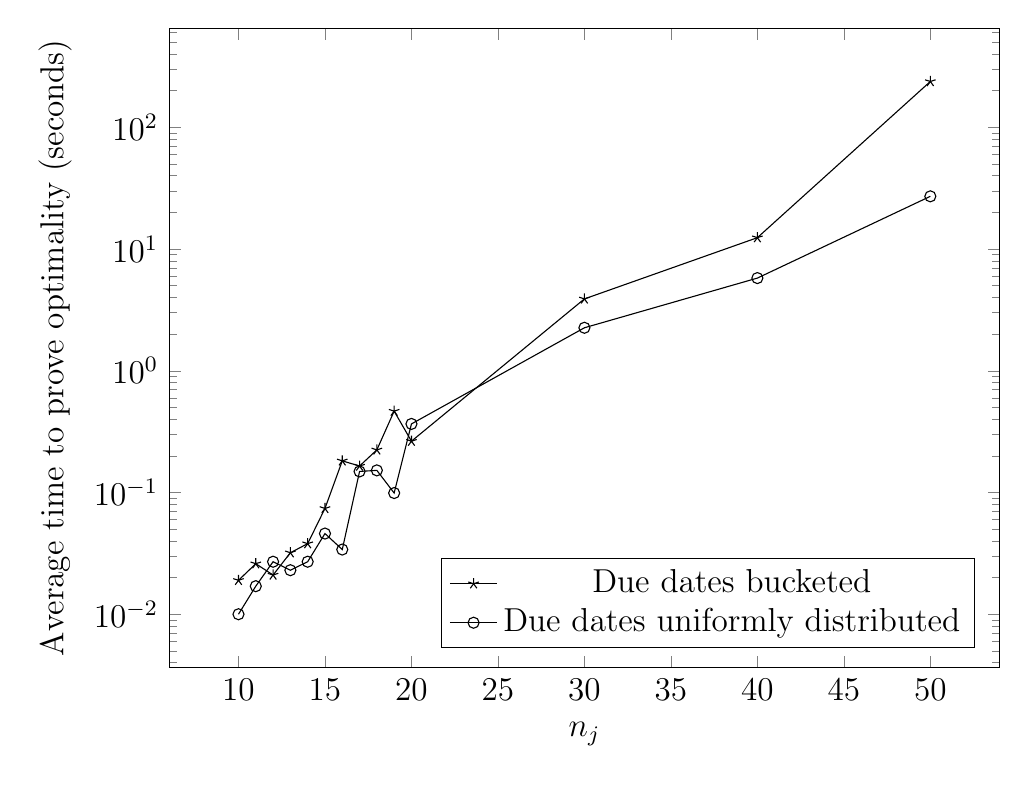
\begin{tikzpicture}
  \begin{semilogyaxis}[xlabel=$n_j$, ylabel=Average time to prove optimality (seconds), width=\textwidth,
  height=0.8\textwidth,legend pos=south east]
    \addplot[color=black, mark=star] coordinates {
(10, 0.019)
(11, 0.026)
(12, 0.021)
(13, 0.032)
(14, 0.038)
(15, 0.074)
(16, 0.182)
(17, 0.165)
(18, 0.224)
(19, 0.466)
(20, 0.264)
(30, 3.895)
(40, 12.403)
(50, 238)
};
  \addlegendentry{Due dates bucketed}
  \addplot[color=black, mark=o] coordinates {
(10, 0.01)
(11, 0.017)
(12, 0.027)
(13, 0.023)
(14, 0.027)
(15, 0.046)
(16, 0.034)
(17, 0.149)
(18, 0.152)
(19, 0.099)
(20, 0.366)
(30, 2.256)
(40, 5.775)
(50, 27.115)
};
  \addlegendentry{Due dates uniformly distributed}
  \end{semilogyaxis}
\end{tikzpicture}

\caption{Comparison of time to prove optimality required by the move-based MIP
model depending on the distribution of due dates.}
\label{fig:uniformddtimecor}
\end{figure}

 Indeed, average performance improves with uniformly distributed due dates on
instances with larger $n_j$.

%%%%%%%%%%%%%%%%%%%%%%%%%%%%%%%%%%%%%%%%%%%%%%%%%%%%%%%%%%%%%%%%%%%%%%%%%%%%
%%%%%%%%%%%%%%%%%%%%%%%%%%%%%%%%%%%%%%%%%%%%%%%%%%%%%%%%%%%%%%%%%%%%%%%%%%%%
%%%%%%%%%%%%%%%%%%%%%%%%%%%%%%%%%%%%%%%%%%%%%%%%%%%%%%%%%%%%%%%%%%%%%%%%%%%%
%%%%%%%%%%%%%%%%%%%%%%%%%%%%%% CONCLUSION %%%%%%%%%%%%%%%%%%%%%%%%%%%%%%%%%%
%%%%%%%%%%%%%%%%%%%%%%%%%%%%%%%%%%%%%%%%%%%%%%%%%%%%%%%%%%%%%%%%%%%%%%%%%%%%
%%%%%%%%%%%%%%%%%%%%%%%%%%%%%%%%%%%%%%%%%%%%%%%%%%%%%%%%%%%%%%%%%%%%%%%%%%%%
%%%%%%%%%%%%%%%%%%%%%%%%%%%%%%%%%%%%%%%%%%%%%%%%%%%%%%%%%%%%%%%%%%%%%%%%%%%%
%%%%%%%%%%%%%%%%%%%%%%%%%%%%%%%%%%%%%%%%%%%%%%%%%%%%%%%%%%%%%%%%%%%%%%%%%%%%

%% TODO
% My new model is better because it's simpler
% It also improves in long time scales, not short ones.
% Could maybe be copied to CP or to similar problems

\chapter{Conclusion}\label{sec:futurework}
The problem of scheduling jobs of non-identical sizes and processing times on a
batch resource with a limited capacity arises frequently in the context of
furnaces, autoclaves, driers, or other machinery where one particular job
determines the processing time of the entire batch. The problem of minimizing
the maximum lateness is given in situations in which all customers (or
downstream processes) are to be treated as fairly as possible.

The problem was approached by Daste \citet{Daste1} using a branch-and-price
model and by Malapert \citet{Malapert} using a new \texttt{sequenceEDD} global
constraint. In this paper we have introduced a set of improvements to Malapert's
basic MIP model, a simple CP model, a decomposition method, and a new MIP based
on the idea of independent search moves expressed in a single formulation.

The new move-based MIP model rivals the performance of Malapert's
\texttt{sequenceEDD} constraint particularly with larger problem instances ($n_j
> 30$). The great simplicity of our formulation allows production managers to
integrate it into existing models without having to implement highly
problem-specific filtering rules. Furthermore, it is easily extended with
additional redundant or lazy constraints if necessary.

\section{Future Work}
All models described in this paper have weaknesses. The improved original MIP
model lacks the fine-tuning and lazy constraints enjoyed by the move-based MIP.
The CP model could likely benefit from additional redundant constraints. The
decomposition approach needs a better pruning method. The move-based MIP's lazy
constraints could certainly be fine-tuned based on a more generous definition of
safe moves and conditional activation relying on the problem's
\textit{disjunction ratio}. Such potential improvements are described in
Appendix \ref{appendix:improvements}.

\subsection{Application to related problems}
The promising computational performance of the move-based MIP model might find
application in similar problems, e.g. completion-time minimization on batch
machines (which is equivalent to $\Lmax$ minimization with equal due dates), or
$\Lmax$ minimization with release dates (i.e. coupling $x_{jk}$ to batch start
times, which can be expressed using an exact analogue to constraint
\eqref{mbm:eq4}).



\bibliographystyle{plainnat}
\bibliography{bibliography}{}
\vskip 4em
\appendix
\chapter[Appendix: Potential improvements to the models]{Appendix: Potential\\ improvements to the models}
\label{appendix:improvements}
The following section details some redundant constraints, tighter variable
bounds and potential fine-tuning opportunities that were not implemented in this
paper, but may be of use in further research. 

\section{CP Model} 
\subsection[Constraint on the number of batches with length $P_k >
p$]{Constraint on number of batches with length {\sansitalicfont
P\textsubscript{k}} > {\sansitalicfont p}}

Since batches take on the processing time of their longest job, there is at
least one batch with $P = \underset{j}{\max} p_j $. We can proceed to fill batches with jobs, ordered by non-increasing processing
time, based on algorithm \ref{alg:findBatchlengthCards}. 

\begin{algorithm}[h!]
\fontsize{9pt}{11.5pt}\selectfont \begin{algorithmic} \State $J^{\star} \gets J$
\Comment{initialize all jobs as unassigned jobs} \State $n_k \gets 1$; $S_k
\gets \{0\}$; $P_{k,\text{min}} \gets \{0\}$ \Comment{Create one empty batch of
size and length zero} \State sort $J^{\star}$ by processing time, non-increasing
\Repeat \State $j \gets J^{\star}$.pop() \Comment{select job for assignment,
longest job first} \Loop $\;$ through all $n_k$ existing batches $k$, first
batch first \State $k_p \gets \emptyset$ \Comment{no feasible batch} \State
$c_\text{min} = b$ \Comment{currently known minimum remaining capacity} \If{$s_j
< b-S_k$ and $b-S_k < c_\text{min}$} \State $k_p \gets k_p$; $c_\text{min} \gets
b-S_k$ \EndIf \EndLoop \If{$|k_p| = 1$} \State $S_{k_p} \gets S_{k_p} + s_j$
\Comment{assign job $j$ to batch $k_p$} \Else \If{$n_k < LB(n_k)$} \State $n_k
\gets n_k + 1$\Comment{open new batch} \State $S_{n_k} \gets s_j$;
$P_{n_k,\text{min}} \gets p_j$ \Comment{assign $s_j$ and $p_j$ to the new batch}
\Else \State leave the loop now and end.  \EndIf \EndIf \Until{$J^{\star}$ is
empty} \end{algorithmic} \caption{Generating lower bounds on batch lengths}
\label{alg:findBatchlengthCards} \end{algorithm}
At the end of this algorithm, we can state: \begin{alignat}{2} &
\mathtt{globalCardinality}(\{1,\dots,n_j\},
\{P_{k,\text{min}}, \dots, P_{k-1,\text{min}} - 1\}, P_k) \quad && \forall k \in \{k_0,\dots,k_{LB(n_k)}\}, \end{alignat}
where the constraint takes three arguments (\mathtt{cards}, \mathtt{vals} and \mathtt{vars}) and $P_{k,\text{min}}$ denotes the minimum length of batch $k$.

The algorithm sorts jobs by non-increasing $p$, and then fills batches job by
job. If a job fits into a previous batch, it is assigned there. If a job fits
into multiple previous batches, it is assigned to the batch with the smallest
remaining capacity. This is called \textit{best-fit decreasing} rule,
and works as follows: let $J^\star$ be the set of jobs sorted by $p$, then at
least one batch will be as long as the longest job $j^\star_1$. If the next $n$
jobs fit into this batch, then there is at least one batch not shorter than
$j^\star_{n+1}$, and similarly for subsequent batches. 

Unfortunately, the optimal solution may perform better than the packing heuristic in
terms of ``vertical'' ($s_j$) bin packing, and may thus require fewer batches.
We therefore need to find a lower bound $LB(n_k)$ on the number of batches, and
we can only guarantee the first $LB(n_k)$ of the above constraints to hold in
the optimal solution. Finding a true lower bound is a two-dimensional bin
packing problem, which is NP-hard. A possible but naive lower bound is $j_0$,
the number of jobs, ordered by decreasing $s_j$, that can never fit into a batch
together.

\subsection[Constraint on the number of batches with due date $D_k >
d$]{Constraint on number of batches with length {\sansitalicfont
D\textsubscript{k}} > {\sansitalicfont d}}

In a similar fashion, we can determine that the second batch must be due no
later than the earliest-due job $j_{m+1}$ that can \textit{not} fit into the first
batch -- if we sort jobs by due date and fit the earliest $m$ jobs into the first
batch -- and so on for subsequent batches. Once again, since best-fit decreasing
may not perform optimally in terms of ``vertical'' packing, this may not be
valid for batches beyond the known $LB(n_k)$.

\subsection[All-different constraints on $P_k$ and $D_k$]{All-different
constraints on {\sansitalicfont P\textsubscript{k}} and {\sansitalicfont
D\textsubscript{k}}}

Furthermore, if all jobs have different processing times, all batches will have
different processing times as well: \texttt{alldifferent}$(P_k)$. If $m$ out of
$n_j$ jobs have different processing times, we can still enforce
\texttt{k\_alldifferent}$(P_k, m)$. Some work on \texttt{k\_alldifferent}
constraints has been done in \citep{Lardeux}. 

Similarly, we knows that the constraint \texttt{k\_alldifferent}$(D_k, m)$ must
be true if $m$ out of $n_j$ jobs have different due dates.

\section{Decomposition approaches}
\subsection{Potential heuristics}
\paragraph{Improve the initial $L_{\text{max,incmb}}$} A better initial
upper bound on $\Lmax$ can help prune some branches of the search tree from the
outset. There are several dispatch rules (or maybe other heuristics?) that could
be explored to do this better.
\paragraph{Improve $L_{\text{max,incmb}}$ during search} It may be useful to
use a heuristic like above to ``complete the schedule'' once a promising partial
schedule has been generated. I have yet to identify situations where this is
always helpful.

% fine-tuning of lazy constraints based on disjunction ratio
% fine-tuning of safe-move lazy constraints' conditions based on minimum
% latenesses for batches.

\section{Move-based MIP model}
\subsection{Conditional activation of lazy constraints}
The disjunction ratio measure introduced by \citet{baptistelepape} may be useful
in conditionally activating or omitting certain lazy constraint sets, as it is
known that they often have a net slowing effect on the solver when dealing with
less difficult problems. This was not implemented for this paper and is thus not
represented in the results in Section \ref{sec:results}, but it certainly has
potential to bring down average solving times, particularly with smaller problem
instances, for which Malapert's \texttt{sequenceEDD} global constraint currently
beats our move-based MIP model.

\subsection[Improvement of \textit{safe move} definition]{Improvement of {\sansitalicfont safe move} definition}
The concept of safe moves is used in several constraints. It describes moves
in which a job $j$ is moved into an earlier batch $k$ and $p_j \leq p_k$.

The definition of safe can be extended to guest jobs $j$ that fulfill the
following condition: $p_j \leq LB(\Lmax) + d_k - UB(S_k)$, where $LB(\Lmax)$ is
a lower bound on the optimal value of $\Lmax$ and $UB(S_k)$ is an upper bound on
the start time of batch $k$. The term represents the longest processing time
that batch $k$ can be extended to without violating a known lower bound on the
maximum lateness.

The a-priori computation of upper bounds on batch start times is challenging,
and can only be based on capacity violations (``what is the longest combination of
guest jobs that can be placed into batches up to and including $k$?''), which
will likely make for relatively weak bounds. Nevertheless, a stronger notion of
safe may be beneficial in some instances.

\chapter{Appendix: Other approaches}
\section{Move-back search}
\label{sec:movebackproof}
The following is a proof referenced in Proposition \ref{prop:moveisbetter}, but
it could easily be turned into a standalone local search method that finds good
solutions quickly.

\begin{proposition}
Begin with any EDD schedule (such as the single-EDD schedule). Moving any job
$j$ into an earlier batch $k$ will never shift the position of $\Lmax$ to the
right (into a later bucket).

\begin{proof}
In any partial schedule following EDD, let $k$ be the batch
with maximum lateness $L_k = \Lmax$. If multiple batches have equal lateness
$\Lmax$, let $L_k$ refer to the latest-due of these batches in the schedule. It has processing time $p_k$. Then the lateness of the
batch before $k$ must be $L_{k-1} \geq L_k - p_k$ as a consequence of the EDD
sequencing. Any batch following $k$ can have a lateness no greater than $L_k -
1$.

\begin{alist}
\item{Moving any single job from a batch following $k$ into a batch before $k$ will
worsen $\Lmax$, but not change its position. Such a move is never necessary to
arrive at an optimal solution.}
\item{Moving back any single job from a
batch before $k$ safely\footnote{for the definition of ``safe'' and
``unsafe'' moves, compare Section \ref{sec:dominance-safe}.} will improve $\Lmax$,
but not change its position.}
\item{Moving back a single pre-$k$ job $j$ from a batch
$\beta$ into an earlier batch $\alpha$ unsafely will reduce $L_k$ by
$p_\alpha$; $\Lmax$ may still be in $k$, or it may be found in any batch between
(and including) $\alpha$ and $\beta$, since their lateness
$L_{[\alpha,\dots,\beta]}$ is now increased by $p_j - p_\alpha$.}
\item{If the
max-lateness job $j$ is single itself, it can be moved from $k$ into an earlier
batch $\alpha$. If this is done safely, the batch immediately preceding
$k$ will still have a lateness $L_{k-1} \geq L_k - p_j$. All batches after $k$
will have their lateness reduced by $p_j$, but since their maximum lateness did
not exceed $L_k - 1$ before the move, it will now be at least 1 less than that
of batch $k-1$.}
\item{If the max-lateness job
$j$ was moved back unsafely into a batch $\alpha$, batches between and
including $\alpha$ and $k-1$ now have their lateness increased by $p_j - p_\alpha$,
while batches after $k$ have their lateness decreased by $p_\alpha$. Again,
batch $L_{k-1}$ would exceed the maximum lateness of batches after $k$.}
\end{alist}
This shows that after a sequence of operations in which single jobs are moved into
earlier batches, $\Lmax$ will never shift to the right. 
\end{proof}
\end{proposition}
In fact, this means that all jobs after the $\Lmax$-job in a single-job EDD
schedule can be ignored in the scheduling problem entirely, although this turns
out to be quite inconsequential as that job is often at or near the end of the
single-job EDD schedule, resulting from the fact that $L_{k-1} \geq L_k - p_k$.
By the same token, high-quality solutions often have their $\Lmax$ in an early
batch.

\section{Other attempts to improve performance}
We present two approaches which, independent of the model used, lead to no change
or a worsening of performance in all initial tests despite appearing very
promising at first. They are mentioned here briefly only for the sake of
completeness.

\subsection[Upper bound on $\Lmax$]{Upper bound on {\sansitalicfont L}\textsubscript{max}}
\label{sec:ublmax}
An upper bound on $\Lmax$ can be found a priori by using a dispatch rule to find a
feasible, if not optimal, schedule. Algorithm \ref{alg:ublmax} shows a variant
in which the longest safely-fitting job is selected first. Using the ``best-fit''
heuristic proposed in Malapert's paper (see Section \ref{sec:bestfit}) yields
better bounds with other problem instances, but is not significantly better
overall. 

\begin{algorithm}[h]
\fontsize{9pt}{11.5pt}\selectfont
\begin{algorithmic}
\State Sort jobs $J$ by due non-decreasing due date
\State $x_j = 1 \forall j \in J$  \Comment $x_j = 0$ iff job $j$ is a guest in an earlier batch
\Repeat{\;Select next job $j$ from $J$}
  \If{$x_j = 0$}    \State continue \Comment skip loop and move to next $j$
  \EndIf
  \State $J^\star \gets$ list of all jobs $i$ after $j$ where $p_i \leq p_j$
  \State Sort $J^\star$ by non-increasing processing time and size
  \Repeat{\;Select next job $i$ from $J^\star$}
    \If{$b - s_j - c_j \geq s_i$} \Comment if remaining capacity suffices for $i$
      \State $x_i \gets 0$
      \State $c_j \gets c_j + s_i$
      \State $B_i \gets j$
    \EndIf
    \If{$b \leq c_j + s_j$} \Comment if capacity exceeded
      \State break
    \EndIf
  \Until{$J^\star$ is empty}
\Until{$J$ is empty}

\State $t \gets 0$ \Comment time index
\Repeat{\;Select next job $j$ from $J$}
  \If{$x_j = 1$}
    \State $t \gets t + p_j$
    \If{$t - d_j > UB(\Lmax)$}
      \State $UB(\Lmax) = t - d_j$
    \EndIf
  \EndIf
\Until{$J$ is empty}
\end{algorithmic}
\caption{Dispatch rule to compute an upper bound on $\Lmax$}
\label{alg:ublmax}
\end{algorithm}

\subsection[Bounding the number of batches $n_k$]{Bounding the number of batches
\sansitalicfont n\textsubscript{k}}\label{sec:bounding_nk}
Initially, the number of batches needed is assumed to be equal to the number of
jobs: $n_k = n_j$. Reducing $n_k$ by pre-computing the maximum number of batches
needed shrinks the $x_{jk}$ matrix, and prunes potential search branches in
branch-and-bound decomposition approaches.


\begin{figure}
  \centering
  \begin{subfigure}[b]{0.4\textwidth}
    \centering
    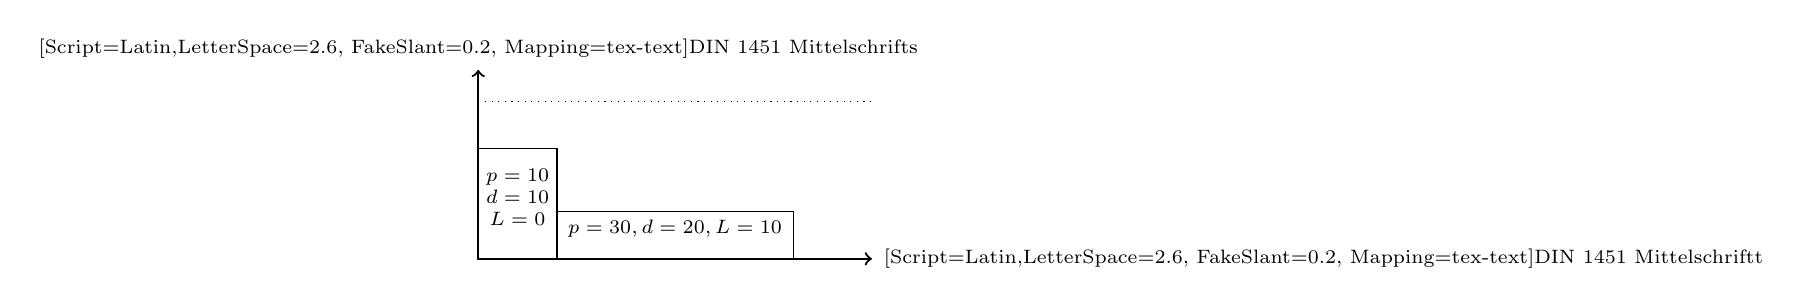
\begin{tikzpicture}[scale=0.2, font=\scriptsize]

      \draw [<->,thick] (0,12) node (yaxis) [above] {\sansitalicfont s}
        |- (25,0) node (xaxis) [right] {\sansitalicfont t};
      \draw[dotted] (0,10) -- (25,10);
        \draw (0,0) rectangle (5,7) node[fn] {$p = 10$\\$d = 10$\\$L = 0$};
        \draw (5,0) rectangle (20, 3) node[fn] {$p = 30, d=20, L=10$};
        
    \end{tikzpicture}
  \end{subfigure}
  \begin{subfigure}[b]{0.4\textwidth}
    \centering
    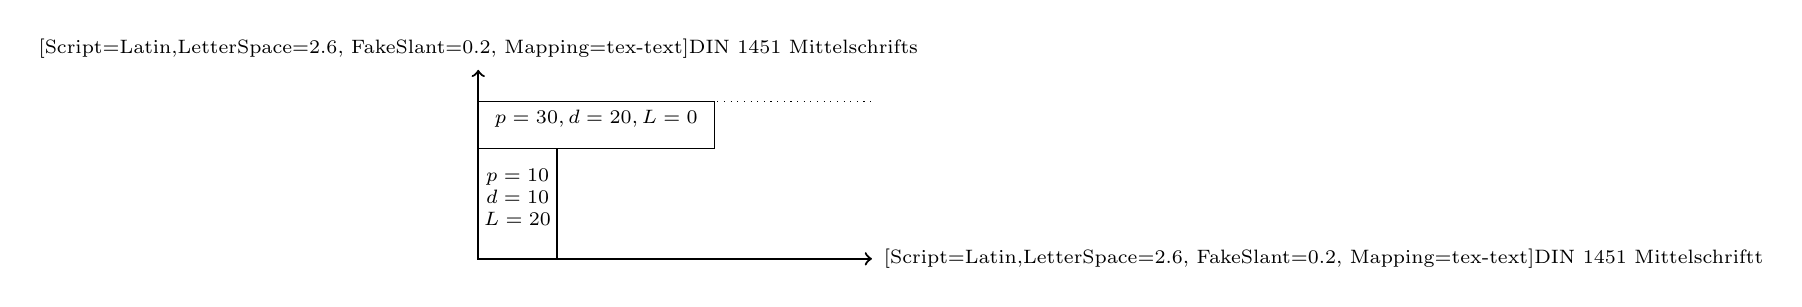
\begin{tikzpicture}[scale=0.2, font=\scriptsize]

      \draw [<->,thick] (0,12) node (yaxis) [above] {\sansitalicfont s}
        |- (25,0) node (xaxis) [right] {\sansitalicfont t};
      \draw[dotted] (0,10) -- (25,10);
        \draw (0,0) rectangle (5,7) node[fn] {$p = 10$\\$d = 10$\\$L = 20$};
        \draw (0,7) rectangle (15, 10) node[fn] {$p = 30, d=20, L=0$};
    
    \end{tikzpicture}
  \end{subfigure}
\caption{Overzealous batch elimination can increase $\Lmax$}\label{fig:bnk1}
\end{figure} %fig:bnk1 (50/10 example)

Unfortunately, we cannot make a general statement that optimal solutions never
have more batches than other feasible solutions -- a simple counterexample is
shown in figure \ref{fig:bnk1}.\footnote{To be more precise, we cannot state
that at least one optimal solution is in the subset of feasible solutions that
uses the fewest number of batches -- a dominance situation that could be
exploited, were it true.}

Starting out with a one-job-per-batch schedule sorted by EDD, we can explore
all feasible batch configurations recursively. To generate any other feasible
schedule (including the optimal solution), jobs $j$ are rescheduled (``moved back'')
from their original batch $k_\text{origin}$ into a prior batch
$k_\text{earlier}$. This eliminates $k_\text{origin}$ and requires, of course,
that $k_\text{earlier}$ has sufficient capacity. If the job's processing time
$p_j$ exceeds that of $k_\text{earlier}$, then the lateness of batches between
$k_\text{earlier}$ and $k_\text{origin}$ will increase. The merit of such a move
cannot be judged a priori (unsafe batch elimination; compare ).
Safe eliminations, on the other hand, will never worsen $\Lmax$, and
only they can be considered when bounding $n_k$ a priori.

Algorithm \ref{alg:bounding_nk} outlines a recursive method to find an upper
bound on $n_k$, recognizing safe batch eliminations only.

\begin{algorithm}[h]
\fontsize{9pt}{11.5pt}\selectfont
\begin{algorithmic}
\If{no open jobs left} \Comment{if this is a ``leaf node'' in the recursion}
  \State update UB$(n_k)$
\EndIf
\State find the combination of unsafe later jobs that fills up the capacity
most, leaving us with capacity $b_r$ 
\State find all combinations $x$ of safe later jobs that fit into $b_r$
\Repeat
  \State $x$ = next safe job combination
  \State \textit{ignoreJobs} $\gets x$ \Comment{make the moves, let the next recursion
  level deal with the rest of the jobs}
  \State spawn and run child node with $J \setminus$ \textit{ignoreJobs}
  \State \textit{ignoreJobs} $\gets$ \textit{ignoreJobs} $\setminus x$
\Until{all combinations have been explored}
\State return
\end{algorithmic}
\caption{Recursive algorithm to find an upper bound on $n_k$}
\label{alg:bounding_nk}
\end{algorithm}

This algorithm evidently requires exponential time. A relaxed variant is a
possible option: if only a single unsafe move \textit{into} a batch is possible,
no safe eliminations into that batch are considered at all and we skip to the
next batch. This would greatly speed up the recursion but also significantly
weaken the usefulness of the resulting upper bound.

In a branch-and-bound decomposition approach in which batches are modelled
individually, an upper bound on $n_k$ could be used to limit the depth of the
search tree, or, in combination with a method to determine a lower bound on the
remaining jobs' $n_k$ at every node, to actively prune the search tree during
the search. The latter method, however, would also run in exponential time as
it, again, would require knapsack-type reasoning unless we use a much less powerful
relaxation.

Another application of a bounded $n_k$ works as follows: a model (CP or MIP) is
somehow optimized to quickly find the optimal solution of a problem that has a
fixed number of batches $n_k \leq n_j$. The model is run with $n_k = n_j$, then
with $n_k = n_j - 1$, then with $n_k = n_j - 2$ etc., until the value of $\Lmax$
starts to increase (which happens at the point where an exceedingly low $n_k$
forces capacity constraints to take precedence over optimality). With every
successive run (i.e. with every decrement of $n_k$), the result of the previous
run is passed to the solver as an initial solution to speed up the search---on
the assumption that job-to-batch assignments will not vary substantially between
runs.

We performed some such tests with a modification of Malapert's original MIP
model. While passing initial solutions to the MIP solver greatly sped up the
search for the optimal schedule at a given $n_k$, the overall time required to
find the optimal solution to a problem instance was significantly greater. We
therefore did not explore this approach further.

\chapter{Appendix: Tabulated results}
\label{appendix:results}
The following table lists solving time for all test instances.

\tiny
\begin{multicols}{5}
\begin{tabular}{c c r}
\toprule
$n_j$ & $i$ & $t$ (seconds) \\
\midrule 
10 & 1 & 0.02 \\
10 & 2 & 0.01 \\
10 & 3 & 0.02 \\
10 & 4 & 0.01 \\
10 & 5 & 0.01 \\
10 & 6 & 0.05 \\
10 & 7 & 0.02 \\
10 & 8 & 0.02 \\
10 & 9 & 0 \\
10 & 10 & 0.03 \\
10 & 11 & 0.02 \\
10 & 12 & 0.02 \\
10 & 13 & 0.01 \\
10 & 14 & 0.02 \\
10 & 15 & 0.02 \\
10 & 16 & 0.01 \\
10 & 17 & 0.02 \\
10 & 18 & 0.02 \\
10 & 19 & 0.01 \\
10 & 20 & 0 \\
10 & 21 & 0.01 \\
10 & 22 & 0.02 \\
10 & 23 & 0.02 \\
10 & 24 & 0 \\
10 & 25 & 0.04 \\
10 & 26 & 0.03 \\
10 & 27 & 0.02 \\
10 & 28 & 0.01 \\
10 & 29 & 0.01 \\
10 & 30 & 0.01 \\
10 & 31 & 0.01 \\
10 & 32 & 0.01 \\
10 & 33 & 0.01 \\
10 & 34 & 0.01 \\
10 & 35 & 0.01 \\
10 & 36 & 0.01 \\
10 & 37 & 0.01 \\
10 & 38 & 0.02 \\
10 & 39 & 0.03 \\
10 & 40 & 0.01 \\
11 & 1 & 0.04 \\
11 & 2 & 0.03 \\
11 & 3 & 0.01 \\
11 & 4 & 0.04 \\
11 & 5 & 0 \\
11 & 6 & 0.04 \\
11 & 7 & 0.03 \\
11 & 8 & 0.01 \\
11 & 9 & 0.03 \\
11 & 10 & 0.03 \\
\bottomrule
\end{tabular}
\vfill
\columnbreak
\begin{tabular}{c c r}
\toprule
$n_j$ & $i$ & $t$ (seconds) \\
\midrule 
12 & 1 & 0.01 \\
12 & 2 & 0.05 \\
12 & 3 & 0 \\
12 & 4 & 0.05 \\
12 & 5 & 0.02 \\
12 & 6 & 0.02 \\
12 & 7 & 0 \\
12 & 8 & 0.02 \\
12 & 9 & 0.02 \\
12 & 10 & 0.02 \\
13 & 1 & 0.04 \\
13 & 2 & 0.03 \\
13 & 3 & 0.08 \\
13 & 4 & 0.01 \\
13 & 5 & 0.07 \\
13 & 6 & 0.02 \\
13 & 7 & 0.02 \\
13 & 8 & 0.01 \\
13 & 9 & 0.02 \\
13 & 10 & 0.02 \\
14 & 1 & 0.02 \\
14 & 2 & 0.08 \\
14 & 3 & 0.07 \\
14 & 4 & 0.06 \\
14 & 5 & 0.02 \\
14 & 6 & 0.04 \\
14 & 7 & 0.03 \\
14 & 8 & 0.02 \\
14 & 9 & 0.01 \\
14 & 10 & 0.03 \\
15 & 1 & 0.03 \\
15 & 2 & 0.07 \\
15 & 3 & 0.01 \\
15 & 4 & 0.04 \\
15 & 5 & 0.03 \\
15 & 6 & 0.01 \\
15 & 7 & 0.07 \\
15 & 8 & 0.37 \\
15 & 9 & 0.04 \\
15 & 10 & 0.07 \\
16 & 1 & 0.05 \\
16 & 2 & 0.03 \\
16 & 3 & 0.07 \\
16 & 4 & 0.17 \\
16 & 5 & 0.23 \\
16 & 6 & 0 \\
16 & 7 & 0.04 \\
16 & 8 & 0.13 \\
16 & 9 & 0.08 \\
16 & 10 & 1.02 \\
\bottomrule
\end{tabular}
\vfill
\columnbreak
\begin{tabular}{c c r}
\toprule
$n_j$ & $i$ & $t$ (seconds) \\
\midrule 
17 & 1 & 0.07 \\
17 & 2 & 0.06 \\
17 & 3 & 0.03 \\
17 & 4 & 1.07 \\
17 & 5 & 0.01 \\
17 & 6 & 0.07 \\
17 & 7 & 0.07 \\
17 & 8 & 0.11 \\
17 & 9 & 0.06 \\
17 & 10 & 0.1 \\
18 & 1 & 0.14 \\
18 & 2 & 0.09 \\
18 & 3 & 0.84 \\
18 & 4 & 0.2 \\
18 & 5 & 0.13 \\
18 & 6 & 0.25 \\
18 & 7 & 0.04 \\
18 & 8 & 0.26 \\
18 & 9 & 0.26 \\
18 & 10 & 0.03 \\
19 & 1 & 0.07 \\
19 & 2 & 0.16 \\
19 & 3 & 0.07 \\
19 & 4 & 0.08 \\
19 & 5 & 0.18 \\
19 & 6 & 0.17 \\
19 & 7 & 1.23 \\
19 & 8 & 0.04 \\
19 & 9 & 2.29 \\
19 & 10 & 0.37 \\
20 & 1 & 0.19 \\
20 & 2 & 0.43 \\
20 & 3 & 0.15 \\
20 & 4 & 0.46 \\
20 & 5 & 0.09 \\
20 & 6 & 0.02 \\
20 & 7 & 1.07 \\
20 & 8 & 0.08 \\
20 & 9 & 0.06 \\
20 & 10 & 0.07 \\
20 & 11 & 0.33 \\
20 & 12 & 1.46 \\
20 & 13 & 1.58 \\
20 & 14 & 0.18 \\
20 & 15 & 0.05 \\
20 & 16 & 0.08 \\
20 & 17 & 0.35 \\
20 & 18 & 0.45 \\
20 & 19 & 1.65 \\
20 & 20 & 0.27 \\
\bottomrule
\end{tabular}
\vfill
\columnbreak
\begin{tabular}{c c r}
\toprule
$n_j$ & $i$ & $t$ (seconds) \\
\midrule 
20 & 21 & 0.81 \\
20 & 22 & 0.31 \\
20 & 23 & 0.13 \\
20 & 24 & 0.15 \\
20 & 25 & 1.47 \\
20 & 26 & 0.15 \\
20 & 27 & 0.08 \\
20 & 28 & 1.57 \\
20 & 29 & 0.05 \\
20 & 30 & 0.14 \\
20 & 31 & 0.13 \\
20 & 32 & 0.07 \\
20 & 33 & 1.33 \\
20 & 34 & 0.52 \\
20 & 35 & 0.23 \\
20 & 36 & 0.21 \\
20 & 37 & 1.08 \\
20 & 38 & 1.56 \\
20 & 39 & 0.37 \\
20 & 40 & 0.69 \\
30 & 1 & 1.68 \\
30 & 2 & 2.35 \\
30 & 3 & 3.15 \\
30 & 4 & 1.93 \\
30 & 5 & 15.13 \\
30 & 6 & 0.37 \\
30 & 7 & 10.31 \\
30 & 8 & 1.88 \\
30 & 9 & 1.68 \\
30 & 10 & 0.47 \\
40 & 1 & 3.77 \\
40 & 2 & 8.3 \\
40 & 3 & 13.34 \\
40 & 4 & 2.88 \\
40 & 5 & 3.63 \\
40 & 6 & 3.31 \\
40 & 7 & 11.43 \\
40 & 8 & 28.39 \\
40 & 9 & 46.56 \\
40 & 10 & 2.42 \\
50 & 1 & 53.8 \\
50 & 2 & 10.15 \\
50 & 3 & 483 \\
50 & 4 & 9.27 \\
50 & 5 & 7.58 \\
50 & 6 & 5.29 \\
50 & 7 & 23.14 \\
50 & 8 & 26.82 \\
50 & 9 & 955.95 \\
50 & 10 & 805.26 \\
\bottomrule
\end{tabular}
\vfill
\columnbreak
\begin{tabular}{c c r}
\toprule
$n_j$ & $i$ & $t$ (seconds) \\
\midrule 
50 & 11 & 6.87 \\
50 & 12 & 5.86 \\
50 & 13 & 7.32 \\
50 & 14 & 57.67 \\
50 & 15 & 9.5 \\
50 & 16 & 9.07 \\
50 & 17 & 5.94 \\
50 & 18 & >3600 \\
50 & 19 & 12.83 \\
50 & 20 & 17.52 \\
50 & 21 & 11.62 \\
50 & 22 & 8.39 \\
50 & 23 & 7.28 \\
50 & 24 & 10.39 \\
50 & 25 & 90.64 \\
50 & 26 & 65.73 \\
50 & 27 & 3.52 \\
50 & 28 & 133.33 \\
50 & 29 & 53.53 \\
50 & 30 & 6.96 \\
50 & 31 & 6.54 \\
50 & 32 & 28.05 \\
50 & 33 & 22.03 \\
50 & 34 & 57.56 \\
50 & 35 & 30.32 \\
50 & 36 & 6.48 \\
50 & 37 & 51.56 \\
50 & 38 & 6.74 \\
50 & 39 & 10.4 \\
50 & 40 & 54.09 \\
\bottomrule
\end{tabular}
\end{multicols}

\section{Results with disjunctiveness measure}

\begin{tabular}{c c r r r}
\toprule
$n_j$ & $i$ & $t$ (s) & $n_j/n_k$ & Disjunction ratio \\
\midrule
30&1&1.84&1.875&0.407777777778\\
30&2&2.45&1.875&0.446666666667\\
30&3&3.3&2&0.347777777778\\
30&4&2.14286&2&0.337777777778\\
30&5&15.56&2.30769&0.296666666667\\
30&6&0.44&1.5&0.583333333333\\
30&7&10.33&2.14286&0.272222222222\\
30&8&1.99&1.76471&0.398888888889\\
30&9&1.78&1.6666&0.502222222222\\
30&10&0.51&1.5&0.584444444444\\
30&11&1.15&1.666667&0.536666666667\\
30&12&2.34&1.875&0.427777777778\\
30&13&1.9&1.66667&0.538888888889\\
30&14&2.73&2&0.346666666667\\
30&15&11.56&2.14286&0.311111111111\\
30&16&2.09&1.66667&0.512222222222\\
30&17&0.89&1.6667&0.524444444444\\
30&18&0.75&1.57895&0.558888888889\\
30&19&0.09&1.42857&0.648888888889\\
30&20&2.36&2&0.397777777778\\
30&21&1.76&1.66667&0.478888888889\\
30&22&2.35&2&0.364444444444\\
30&23&0.67&1.76471&0.487777777778\\
30&24&1.11&1.76471&0.471111111111\\
30&25&3.83&2.14286&0.297777777778\\
30&26&3.59&2&0.354444444444\\
30&27&7.32&2.30769&0.251111111111\\
30&28&1.71&2&0.362222222222\\
30&29&6.82&2&0.294444444444\\
30&30&0.41&1.5&0.671111111111\\
30&31&1.29&1.76471&0.516666666667\\
30&32&2.62&1.875&0.428888888889\\
30&33&2.15&2&0.395555555556\\
30&34&2.44&1.76471&0.392222222222\\
30&35&4.86&2&0.312222222222\\
30&36&1.53&2&0.37\\
30&37&4.23&2.14286&0.297777777778\\
30&38&1.43&1.57895&0.525555555556\\
30&39&1.2&1.875&0.348888888889\\
30&40&1.45&1.76471&0.362222222222\\
\bottomrule
\end{tabular}
\pagebreak
\section{Results with non-bucketed job due dates}
\begin{multicols}{4}
\begin{tabular}{c c r}
\toprule
$n_j$ & $i$ & $t$ (seconds) \\
\midrule 
10 & 1 & 0.01 \\
10 & 2 & 0 \\
10 & 3 & 0 \\
10 & 4 & 0 \\
10 & 5 & 0.01 \\
10 & 6 & 0.04 \\
10 & 7 & 0.01 \\
10 & 8 & 0.02 \\
10 & 9 & 0.01 \\
10 & 10 & 0 \\
11 & 1 & 0.01 \\
11 & 2 & 0.02 \\
11 & 3 & 0.01 \\
11 & 4 & 0.02 \\
11 & 5 & 0 \\
11 & 6 & 0 \\
11 & 7 & 0.03 \\
11 & 8 & 0.01 \\
11 & 9 & 0.06 \\
11 & 10 & 0.01 \\
12 & 1 & 0.04 \\
12 & 2 & 0.05 \\
12 & 3 & 0.02 \\
12 & 4 & 0.04 \\
12 & 5 & 0.02 \\
12 & 6 & 0.02 \\
12 & 7 & 0.01 \\
12 & 8 & 0.02 \\
12 & 9 & 0.01 \\
12 & 10 & 0.04 \\
13 & 1 & 0.01 \\
13 & 2 & 0.03 \\
13 & 3 & 0.03 \\
13 & 4 & 0.01 \\
13 & 5 & 0.01 \\
\bottomrule
\end{tabular}
\vfill
\columnbreak
\begin{tabular}{c c r}
\toprule
$n_j$ & $i$ & $t$ (seconds) \\
\midrule 
13 & 6 & 0.07 \\
13 & 7 & 0 \\
13 & 8 & 0.02 \\
13 & 9 & 0.01 \\
13 & 10 & 0.04 \\
14 & 1 & 0.02 \\
14 & 2 & 0.02 \\
14 & 3 & 0.01 \\
14 & 4 & 0.09 \\
14 & 5 & 0.03 \\
14 & 6 & 0.01 \\
14 & 7 & 0.03 \\
14 & 8 & 0 \\
14 & 9 & 0 \\
14 & 10 & 0.06 \\
15 & 1 & 0.01 \\
15 & 2 & 0.11 \\
15 & 3 & 0.05 \\
15 & 4 & 0.04 \\
15 & 5 & 0.02 \\
15 & 6 & 0.05 \\
15 & 7 & 0.05 \\
15 & 8 & 0.06 \\
15 & 9 & 0.02 \\
15 & 10 & 0.05 \\
16 & 1 & 0.01 \\
16 & 2 & 0.04 \\
16 & 3 & 0.02 \\
16 & 4 & 0.02 \\
16 & 5 & 0.08 \\
16 & 6 & 0.01 \\
16 & 7 & 0.04 \\
16 & 8 & 0.05 \\
16 & 9 & 0.01 \\
16 & 10 & 0.06 \\
\bottomrule
\end{tabular}
\vfill
\columnbreak
\begin{tabular}{c c r}
\toprule
$n_j$ & $i$ & $t$ (seconds) \\
\midrule 
17 & 1 & 0.03 \\
17 & 2 & 0.1 \\
17 & 3 & 0.02 \\
17 & 4 & 0.21 \\
17 & 5 & 0.18 \\
17 & 6 & 0.04 \\
17 & 7 & 0.01 \\
17 & 8 & 0.67 \\
17 & 9 & 0.12 \\
17 & 10 & 0.11 \\
18 & 1 & 0.07 \\
18 & 2 & 0.13 \\
18 & 3 & 0.05 \\
18 & 4 & 0.03 \\
18 & 5 & 0.79 \\
18 & 6 & 0.1 \\
18 & 7 & 0.01 \\
18 & 8 & 0.05 \\
18 & 9 & 0.1 \\
18 & 10 & 0.19 \\
19 & 1 & 0.08 \\
19 & 2 & 0.05 \\
19 & 3 & 0.24 \\
19 & 4 & 0.04 \\
19 & 5 & 0.11 \\
19 & 6 & 0.04 \\
19 & 7 & 0.18 \\
19 & 8 & 0.03 \\
19 & 9 & 0.08 \\
19 & 10 & 0.14 \\
20 & 1 & 0.06 \\
20 & 2 & 0.5 \\
20 & 3 & 0.03 \\
20 & 4 & 0.15 \\
20 & 5 & 1.45 \\
\bottomrule
\end{tabular}
\vfill
\columnbreak
\begin{tabular}{c c r}
\toprule
$n_j$ & $i$ & $t$ (seconds) \\
\midrule 
20 & 6 & 0.3 \\
20 & 7 & 0.13 \\
20 & 8 & 0.67 \\
20 & 9 & 0.22 \\
20 & 10 & 0.15 \\
30 & 1 & 3.8 \\
30 & 2 & 7.38 \\
30 & 3 & 1.68 \\
30 & 4 & 3.35 \\
30 & 5 & 0.9 \\
30 & 6 & 0.27 \\
30 & 7 & 0.6 \\
30 & 8 & 0.59 \\
30 & 9 & 0.27 \\
30 & 10 & 3.72 \\
40 & 1 & 2.06 \\
40 & 2 & 2.2 \\
40 & 3 & 7.63 \\
40 & 4 & 3.15 \\
40 & 5 & 1.99 \\
40 & 6 & 1.65 \\
40 & 7 & 6.05 \\
40 & 8 & 2.28 \\
40 & 9 & 16.92 \\
40 & 10 & 13.82 \\
50 & 1 & 7.27 \\
50 & 2 & 3.31 \\
50 & 3 & 41.67 \\
50 & 4 & 16.9 \\
50 & 5 & 12.75 \\
50 & 6 & 6.24 \\
50 & 7 & 7.32 \\
50 & 8 & 34.12 \\
50 & 9 & 8.89 \\
50 & 10 & 132.68 \\
\bottomrule
\end{tabular}
\end{multicols}


\backmatter
\pagebreak
\thispagestyle{empty}
\vspace*{\fill}
\end{document}

